\documentclass[a4paper, 12pt, twoside]{report}

\usepackage[top=2.5cm, bottom=3cm, left=3cm, right=2cm]{geometry}
\usepackage{mathtools}
\usepackage{amsthm}
\usepackage[bitstream-charter]{mathdesign}
\usepackage[pdftex]{graphicx}
\usepackage{fixltx2e}
\usepackage{afterpage}
\usepackage{latexsym}
\usepackage{times}
\usepackage{amsmath}
\usepackage{subfigure}
\usepackage{multirow}
\usepackage{rotating}
\usepackage[table]{xcolor}
\usepackage{setspace}
\usepackage[nottoc]{tocbibind}

\usepackage{setspace}
\usepackage{xcolor}
\usepackage{natbib}
\usepackage{enumitem}

\usepackage[acronym, toc]{glossaries}
\usepackage[toc, page]{appendix}

\usepackage{tikz}
\usetikzlibrary{shapes.geometric, arrows}

\usepackage{color}
\definecolor{myColLnk}{HTML}{0000FF}
\definecolor{myColUrl}{HTML}{0F0FFF}

\usepackage{hyperref}
\hypersetup{
	colorlinks = true,	% make the links colored
	linkcolor = myColLnk,		% color TOC links in blue
	urlcolor = myColUrl,		% color URLs in ___
	linktoc = all		% 'all' will create links for everything in the TOC
}

\newcommand{\q}[1]{``#1''}
\newcommand{\HRule}{\rule{\linewidth}{0.5mm}}
\newcommand{\scDiaeresis}[1]{\"{#1}}
\newcommand{\algoTab}{\hspace*{1cm}}
\newcommand{\myTab}{\hspace*{4em}}

\newenvironment{dedication}
{
	\clearpage		% we want a new page
	\thispagestyle{empty}	% no header and footer
	\vspace*{\stretch{1}}	% some space at the top
	\itshape		% the text is in italics
	\centering		% flush to the right margin
}
{
	\par			% end the paragraph
	\vspace{\stretch{3}}	% space at bottom is three times that at the top
	\clearpage		% finish off the page
}
\newtheorem{theorem}{Theorem}
\newtheorem{remark}{Remark}
\newtheorem{definition}{Definition}
\newtheorem{corollary}{Corollary}
\newtheorem{lemma}{Lemma}
\newtheorem{note}{Note}

\makeglossaries
\newglossaryentry{blockchain}{
	name = BlockChain,
	description = {A chain database of blocks of data created after blocks being verified by most members of the network}
}

\newacronym{gcd}{GCD}{Greatest Common Divisor}


\setcounter{tocdepth}{3}
\setcounter{secnumdepth}{3}

\tikzstyle{startstop} = [rectangle, rounded corners, minimum width=3cm, minimum height=1cm, text centered, draw=black, fill=red!30]
\tikzstyle{io} = [trapezium, trapezium left angle=70, trapezium right angle=110, minimum width=3cm, minimum height=1cm, text centered, draw=black, fill=blue!30]
\tikzstyle{pl} = [rectangle, rounded corners, minimum width=1cm, minimum height=1.5cm, text centered, draw=black, fill=red!30]
\tikzstyle{node} = [circle, text centered, draw=black, fill=blue!30]
\tikzstyle{process} = [rectangle, minimum width=3cm, minimum height=1cm, text centered, draw=black, fill=orange!30]
\tikzstyle{decision} = [diamond, minimum width=3cm, minimum height=1cm, text centered, draw=black, fill=green!30]
\tikzstyle{arrow} = [thick, ->, >=stealth]

\begin{document}
\begin{titlepage}

\begin{center}
\HRule \\[0.4cm]
{\huge \bfseries \textbf{Image Integrity Analysis with BlockChain Technology}  \\[0.4cm] }
\HRule \\[1cm]
\end{center}

\vspace{0.2cm}

\begin{center}
{\large{Bachelor Thesis}}
\end{center}

\vspace{0.25cm}

\begin{center}
\large{\textit{Submitted By}}
\end{center}

\vspace{0.35cm}

\begin{center}
{\large{Anuj Kr. Pathak\\\&\\Sayan Shankhari}}
\end{center}

\vspace{0.25cm}

\begin{figure}[h]
\centering
\includegraphics[width=0.25\textwidth]{./img_src/iiitk.png}
\end{figure}

\vspace{0.5cm}

\begin{center}
{\textit{\Large{A thesis submitted to}}} \\
\end{center}

\vspace{0.25cm}

\begin{center}
\Large{Indian Institute of Information Technology Kalyani} \\
\end{center}

\vspace{0.35cm}

\begin{center}
\textit{\large {for the partial fulfillment of the degree of}} \\
\vspace{0.8cm}
\textbf{\Large{Bachelor of Engineering in Computer Science}} \\
\end{center}

\begin{center}
\textbf{{\large{in}}}
\end{center}

%\vspace{0.1cm}
\begin{center}
\textbf{\Large{Department of Computer Science and Information Technology}} \\
\end{center}

\vspace{0.5cm}

\begin{center}
\Large{May, 2019}
\end{center}

\end{titlepage}

\newpage
\begin{dedication}
\textit{To my beloved parents and friends who have supported me and prayed for my success\\ throughout my life.}
\end{dedication}

\newpage
\chapter*{}
%\setcounter{page}{1}
\pagenumbering{roman}
\begin{center}
\textbf{\textsc{\Large Certificate}}\\[0.75cm]
\end{center}

\onehalfspacing This is to certify that the thesis entitled
\textbf{Image Integrity Analysis with BlockChain Technology} being submitted by undergraduate students \textbf{Anuj Kr. Pathak} (Reg. No.: 000000102) and \textbf{Sayan Shankhari} (Reg. No.: 00000121) in the Department of Computer Science and Information Technology, Indian Institute of Information Technology Kalyani, Nodia, 741235, India, for the award of \textbf{Bachelors of Technology} in \textbf{Computer Science \& Engineering}, is an original research work carried by them under my supervision and guidance. The synopsis has fulfilled all the requirements as par the regulation of \textbf{IIIT Kalyani} and in my opinion, has reached the standards needed for submission. The works, techniques and the results presented have not been submitted to any other university or Institute for the award of any other degree or diploma.\\
\bigskip
\bigskip
\bigskip
\bigskip
\bigskip
\bigskip
\bigskip
\begin{flushleft}
\bigskip
-------------------------------\\
(\textbf{Dr. Imon Mukherjee})\\
\smallskip
Assistant Professor\\
Department of Computer Science and Information Systems\\
Indian Institute of Information Technology Kalyani\\
IIIT Kalyani Campus, West Bengal 741235, India.
May 2019\\
\end{flushleft}

\newpage
\chapter*{}
%\setcounter{page}{1}
%\pagenumbering{roman}
\begin{center}
\textbf{\textsc{\Large Declaration}}\\[0.75cm]
\end{center}

\onehalfspacing
We hereby declare that the work being presented in this thesis entitled, \textbf{\q{Image Integrity Analysis with BlockChain Technology}}, submitted to Indian Institute of Information Technology Kalyani in partial fulfilment for the award of the degree of Bachelor of Technology in Computer Science and Engineering during the period from July, 2018 to May, 2019 under the supervision of Dr. Imon Mukherjee, Department of Computer Science and Engineering, Indian Institute of Information Technology Kalyani, West Bengal 741235, India, does not contain any classified information.

\bigskip
\bigskip
\bigskip
\bigskip

\noindent
-------------------------------- \hfill -------------------------------- \\
\textbf{Anuj Kumar Pathak} \hfill \textbf{Sayan Shankhari} \\
39/CSE-15145 :: 00000102 \hfill 67/IT-15026 :: 00000121 \\
Computer Science and Engineering, \hfill Information Technology, \\
Indian Institute of Information \hfill Indian Institute of Information\\
Technology Kalyani, \hfill Technology Kalyani, \\
WEBEL IT Park, West Bengal \hfill WEBEL IT Park, West Bengal \\
741235 India \hfill 741235 India

\bigskip
\bigskip
\bigskip
This is to certify that the above statement made by the candidate is correct to the best of my knowledge.

\bigskip
\begin{flushleft}
\bigskip
\bigskip
------------------------------- \\
(\textbf{Dr. Imon Mukherjee}) \\
\smallskip
Assistant Professor \\
Department of Computer Science and Information Systems \\
Indian Institute of Information Technology Kalyani \\
IIIT Kalyani Campus, West Bengal 741235, India \\
May 2019 \\
\end{flushleft}

\chapter*{Acknowledgments}
First of all, We would like to take this opportunity to thank my supervisor Dr. Imon Mukherjee without whose effort this thesis would not have been possible. We are so grateful to him for working tirelessly after us, clearing our doubts whenever and wherever possible. We are most grateful to Department of Computer Science and Information Technology, Indian Institute of Information Technology Kalyani, West Bengal, 741235, India, for providing us this wonderful opportunity to complete our bachelor thesis. We would like to thank our friends for providing us help as and when required. We would like to thank our team mates for being a great motivators and great friends. \\
\\
\linebreak And last but the biggest of all, We want to thank our parents, for always believing in us and letting us do what we wanted, but keeping a continuous check that we never wandered off the track from my goal. \\

\bigskip
\bigskip
\bigskip
\bigskip

\noindent
-------------------------------- \hfill -------------------------------- \\
\textbf{Anuj Kumar Pathak} \hfill \textbf{Sayan Shankhari} \\
CSE-150\_\_ :: 00000102 \hfill IT-15026 :: 00000121 \\
Computer Science and Engineering, \hfill Information Technology, \\
Indian Institute of Information \hfill Indian Institute of Information\\
Technology Kalyani, \hfill Technology Kalyani, \\
WEBEL IT Park, West Bengal \hfill Webel IT Park, West Bengal \\
741235 India \hfill 741235 India


%\singlespacing
\pagebreak \tableofcontents
\pagebreak \listoffigures

\printglossary[type=\acronymtype]
\printglossary

\newpage
\chapter*{Abstract}
With the digitalization any historical record are available in the form of collection of bits. Any document can be stored in advanced electronic devices like computers, smart phones file systems as files. The most used or popular files are media files (image, audio, video). For the lack of true information and experience or bad ethics of mind the number of digital scams is getting higher in developing country like India. So the data files need to be protected somehow somewhere and also there should be a system that will veryfy the requested file. So we started with the simplest media format \textit{i.e.} Image. Making a centrral database can be unreliable because the system can be breached and the data might be changed no matter how advanced and protective the protocols are. So we took the concept from advanced decentralized architecture of BlockChain mostly BitCoin.
A purely peer-to-peer version of online data would allow online transactions to be sent directly from one node to another without going through a central authority. Digital signatures provide part of the solution.
The network timestamps transactions by hashing them into an ongoing chain of hash-based proof-of-work, forming a record that cannot be changed without redoing the proof-of-work. The longest chain not only serves as proof of the sequence of events witnessed, but proof that it came from the largest pool of CPU power. As long as a majority of CPU power is controlled by nodes that are not cooperating to attack the network, they'll generate the longest chain and outpace attackers. The network itself requires minimal structure. Messages are broadcast on a best effort basis, and nodes can leave and rejoin the network at will, accepting the longest proof-of-work chain as proof of what happened while they were gone.
To prevent the action against one of the biggest issues in India of Fake Media (Image, Sound) Scam. This project tries to find a way to prevent it with a new upcoming technology starting with image files.

\textbf{Keywords:} Peer-to-Peer network, Proof-of-work, Proof-of-Stake, Distributed Ledger, Concensus Mechanism, Hash Function, Video Formatting, Image File formats, Watermarking, WebServer.

% \afterpage{\null\newpage}
\chapter{Introduction}
\label{Ch1}
%\setcounter{page}{1}
\pagenumbering{arabic}

\bigskip
\bigskip
\bigskip

This chapter presents the introduction of the thesis that includes the brief description of BlockChain, and the adopted approach to address the problems. This chapter also presents the scope of this thesis and the contributions of the thesis.

Image integrity is the task of checking if the image file's bits are changed or not at any point. A digital file might change by platforms. This would be fully online system. Nowadays with increasing people in digital world the editing softwares are getting smart. Most of the files that might be non-editable in some operating systems or file systems, but the so called hackers or masters of electronic devices have file systems that can easily access and change any file data. So in that way the media files can not be checked for integrity. And also while the images are shared in different platforms, the files' data might be changed according to their protocols for data compression or security.

The proposed system in this thesis will help us to detect those shared files and compare them not bit by bit, but context wise and signature wise. That means if one shares an image both our system as well as one of those online platforms and download them as separate file and check in our system, it should return truth values if data portion are same or atleast 95\% same. The system we are introducing the social media like platform that have the capability to store images and show them in news feed. There is a option for every photo to download in user's computer or mobile devices and after sharing and getting back the person can check if the file is intact or not in our proposed system by the digital signature.

\section{Scope of Discussion}
This thesis focuses on building a hybrid architechture inspired by one of the major implementations of BlockChain i.e. BitCoin~\cite{nakamoto2008bitcoin}. By the advancement of PHP (Hypertext PreProcessor) and JS (JavaScript) which are the basic building languages or platforms that can be run in any modern devices, it might be quite easy to make a peer-to-peer web-api (Application Programming Interface) running like bitcoin decentraized network as well as social media platform that might be a real Truth Machine. While comparing image files data we will first compress the data using our own protocol and compare by bit matching Euclid, or Deep CNN (Convolutional Neural Network).

\section{Methodological Approach}
The system that we are trying to build is capable of processing, storing and showing image files. Not only that, it also allows viewers to veryfy his own copy of the image. It is not easy to store and veryfy in a moment and it is about impossible to change the whole blockchain, because the miners have their own copy of the public ledger and their processed computation powers in their computers. The automated server should back up its data from both the Virtual miners as well as remote miners' computers. The studied and inspired technologies are discuussed in the thesis.

\section{Thesis Contribution}
The main contributions of this thesis includes
\begin{enumerate}
\item Proposes an user anonymity-preserving algorithm to be a part of Video Integrity Program.
\item Formally analyzes the security of the newly designed protocol as well as its performance.
\item The scheme, as compared to the existing schemes, not only authenticates the users but, also establishes a session key between the user and the System after successful mutual authentication.
\item The scheme provides many security and robustness features of user authentication and Block Processing scheme for BCTs.
\item No installation required to be a part of the system, except you want to be the miner.
\end{enumerate}

\section{Roadmap of the Thesis}
The structure of the thesis is as follows:
\begin{enumerate}
\item The Chapter \ref{Ch1} is an introductory part which discusses the scope of the thesis, about the contribution of this thesis and the motivation for writing it.
\item The Chapter \ref{Ch2} provides the background of Image integrity security aspects of it and previous works.
\item The Chapter \ref{Ch3} introduces the proposed authentication framework after highlighting the motivations behind this work.
\item The implementation of Chapter \ref{Ch5}, where an informal implementation of the proposed protocol has been discussed.
\item The Chapter \ref{Ch6} comprises of the conclusion and further work of the Project in future.
\end{enumerate}

\section{BlockChain}
A BlockChain or \textbf{\q{The Truth Machine}} ~\cite{the_truth_machine} can be broadly described as a peer-to-peer network of nodes that makes a collaborative effort in sensing certain specified chain of blocks of data around its periphery and thereby controls the surrounding environment.
Accrrding to Wikipedia~\cite{blockchain_wiki} a blockchain, originally block-chain, is a growing list of records, called blocks, which are linked using cryptography. Each block contains a cryptographic hash of the previous block, a timestamp, and transaction data (generally represented as a Merkle tree).
In BlockChains, each node consists of processing capability, it may contain multiple types of memory like program, data and memories, having a Web-Service transceiver, Client-side processors, and a power source. The nodes communicate with each other using web-services and self-organized.
There are certain nodes called miners that veryfies each transactions or entry of data in the chain and are the most reliable personnel in the network who always have the updated copy of blocks of data.

\begin{figure}
\begin{center}
\includegraphics[width=0.5\textwidth]{./img_src/blockchain.jpg}
\end{center}
\caption{Overview of Block-Chain Technology (BCTs).}
\end{figure}

Some of the underlying concepts of the BlockChain especially BitCoin (the most popular implementation of BlockChain) and some other important technology are briefed.

\subsection{Peer-to-Peer Network}
This is the internet protocol that connects different logged in users as a node which is having some computation power. The users who are only uploading and verifying may have computer or smartphone, but the verifiers or the miners must have to work on computer with sufficient amount of computation power.

\subsection{Transactions}
Everything in crypto-currency comes under transactions, i.e. someone is sending some amount of money to someone else at some time. So a basic or overall transaction data can be structured as,

\fbox{\colorbox{lightgray}{\parbox[b][4cm][c]{0.50\linewidth}{
\textbf{\texttt{\noindent Transaction :: \{\\
\hspace*{1cm} \textless Transaction\_id\textgreater,\\
\hspace*{1cm} \textless TimeStamp\textgreater,\\
\hspace*{1cm} \textless Sender\_Id\textgreater,\\
\hspace*{1cm} \textless Receiver\_Id\textgreater,\\
\hspace*{1cm} \textless Amount\_Unit\textgreater\\
\noindent \}}}
}}}

This transaction details is send to every peer to verify. If they heard already about it, it is true, or it is false (same as women's un-manipulated gossip in village). If more than 50\% population declare it true, then it is allowed to be in the Public Ledger.

\subsection{Public Ledger}
This is the publicly shared record of transactions kept as a list of blocks. At a particular point of time everybody (every node), who are connected to the network, should have a same copy of ledger in their own devices of what server has. Whenever a new person logs into the network aotomatically the server forces to update the ledger to the person's device. So basically the ledger is the chain file.

\subsection{Chain of Blocks}
It means list of blocks of data having some common part with previous and next block. This is like Single-way linked-list(every node consists of data and program memory address to the next node). Every block contains a number of transactions and many more things.

\fbox{\colorbox{lightgray}{\parbox[b][6cm][c]{0.75\linewidth}{
\textbf{\texttt{\noindent Block :: \{\\
\hspace*{1cm} \textless Block\_Id\textgreater,\\
\hspace*{1cm} \textless TimeStamp\textgreater,\\
\hspace*{1cm} \textless Merkle\_Root\textgreater,\\
\hspace*{1cm} \textless Verifier\_Id\textgreater,\\
\hspace*{1cm} \textless Nonce\_Value\textgreater,\\
\hspace*{1cm} \textless Previous\_Hash\textgreater,\\
\hspace*{1cm} \textless Current\_Hash\textgreater,\\
\hspace*{1cm} \textless Data :: ANumberOfTransactions\textgreater\\
\noindent \}}}
}}}

So it is kind of backword linked-list which is propagating by having the previous block's kind of identity (because there is a mild chance of collision i.e. multiple values' hashes are same) hash.

\subsection{Timestamp}
The time means absolute global date-time in the format: 

\fbox{\colorbox{lightgray}{\parbox[b][2cm][c]{\linewidth}{
\textbf{\texttt{\noindent TimeStamp :: String (
\textless day\_of\_week\_code :: ddd\textgreater,
\textless month\_code :: mmm\textgreater,
\textless day\_of\_month :: dd\textgreater,
\textless year :: yyyy\textgreater,
\textless time :: hh:mm:ss\textgreater,
\textless Distance from Mean-TimeLine :: GMT+hhmm\textgreater,
\textless Time Zone :: Country\_Name Standard Time\textgreater
\noindent )}}
}}}

Example: \textbf{\q{Sat May 25 2019 20:45:04 GMT+0530 (India Standard Time)}}. The timestamp is one of the most needed to prove it later for verification of the record. It is used to create the current block's hash.

\subsection{Hash}
The job of a hash algorithm is to map any size of domain to a particular size of range. SHA-256 is one of the most popular hash algorithms which takes any length input and returns 256 bit output. All input/output operations can be transferred into strings.

\subsection{Merkle Root Hash}
Merkle tree is a complete binary tree which has the hash values of transaction data as leaf nodes. The tree propagation occures from leaves to root as tournament tree form. For any point,

			parent hash = hash(child-1 hash + child-2 hash);

A little change in any data of any transaction will change the merkle root, and thus the block's hash and the complete chain. Because it is used to create the current block's hash.

\subsection{Previous Hash}
The previous block's hash. It is required to maintain the chain system because we can not create the next address and we don't know when it would be created, so it is better to store what we already have. It is used to create the current block's hash.

\subsection{Nonce}
It is the quantity of computation power used to solve a mathematical problem which is not so hard but not so easy either. Too easy solution will be easy to break and too hard solution will take so long time to create a block that the adversary with huge computation power have a chance to alter the data before creating and verifying a block. Rather a medium hard problem will be better. It is used to create the current block's hash.

This is to show the verifiers that the block creator have spent sufficient amount of computation power before creating the block and also to delay the process a little bit and this is called POW (Proof of Work). In bitcoin the problem is to find the first hash of given values which is having 'd' number of leading 'zero's where the 'd' represents the difficulty of the problem i.e. the more 'd' gets it will take longer to calculate. Typical value of 'd' is 32 bits and average delay for the whole block addition (create, verify then add) is about 10 minutes.

\subsection{Consensus Mechanism}
It is the contract or the protocol by which the blocks are verified and the winning blocks are added to everyone's ledger as well as the central server. The actual consensus algorithm is not published for security reasons. But by possible ways or reverse eengineering people have created  different models. Some of those models are:

\begin{figure}
\begin{center}
\includegraphics[width=0.75\textwidth]{./img_src/bitcoin.jpg}
\end{center}
\caption{Overview of BitCoin Technology (BCTs).}
\end{figure}

\begin{enumerate}
\item Probable bitcoin consensus mechanism
\item Paxos (Part-Time Parliament) consensus mechanism~\cite{paxos_made_easy, paxos_made_practical}
\item Raft consensus mechanism~\cite{raft_extd}
\end{enumerate}

Bitcoins one is probably the simplest one, but having bugs. The Paxos allows different types of sources and faults to come, it learns and fixes it. Raft does not allow any fault to happen.

The basic overall way in which consensus happen in bitcoin might be the following,

\begin{enumerate}
\item The transaction comes to server from client nodes;
\item Server stores that in file system database as unverified transaction;
\item At the point of interval of 10 minutes server broadcasts it to the miners network i.e. to every miner;
\item Each miner individually verifies and adds correct transaction in a block. Each node holds its block creation and validates the new block as soon as it gets new block from network. Who's block is valid and introduced first to network will be added to everyone's chain and they will start making new block on top of it. Sometimes forks might be created for the networking distance between distant nodes, at that moment conflict will come. If a new introduced block's previous hash does not match with the last block's current hash the node requests to the network to get the missing blocks one by one until the blocks match, it validates it, delete the wrong blocks (make them orphan) and add missing blocks to own chain to resolve fork and maintain longest updated chain. So it is a race between miner nodes.
\item Server gets a copy from miners group and updates own copy and delete the added tansactions from file system.
\end{enumerate}

\subsection{Applications of BCTs}
Block-Chain Technology provides one major advantage over conventional centralized database system: immunity from unexpected data changes or Hacks, which gives rise to numerous applications. Some of them include

\begin{itemize}
\item Crypto-currency: Creating and transferring digital money, Data Mining.
\item Military applications: Secure and verified records of Every Military Events and documents.
\item Structural health Monitoring
\item e-Biding Systems
\item Election System or e-Voting Systems
\item Selling Records and other Commercial Applications
\item Music Copyright Verification System
\item Integrity Analysis of Media Files
\end{itemize}

\subsection{Security and Integrity in BCTs}
As the data is not sitting on a single data server so there is no security issue for Server Hacking. And also the hash-Chain with Cryptography makes it near to impossible to figure out or change previous data block in the blockchain. Before adding any data block with the help of consensus mechanism the blocks are verified with the digital signature of the node and some solution of nonce (the number of times the cllient application required to calculate the mathematical problem) and various other meta data.
As in some interval the system is refreshing itself, if some error seems to be occured, it backs up itself by contacting the miners (the trusted nodes), compare their files and back up with the valid one. So no integrity problem is there, unless and until the internet works fine.

\chapter{Background}
\label{ch:2}
\bigskip
As we all know that in India the politics and the social media is a big thing for people to consider as an important part of life. But the problem is that some social media users does think of exploiting with the content either by downloading the image or video or recording on screen and uploading it to the social media platforms. Those new images might be very sensitive and controversial and that becomes viral and put bad impact on the society.

The integrity of data has become more and more important. Security breaches that have leaked passwords and user emails are commonplace and regularly appear in the news. When a system is hacked, the first issue that usually comes to mind is the compromise of confidentiality, specifically what confidential information is now in the hands of the adversary.
Another aspect, which is getting increasingly important, is to know the integrity of data, has anything been changed contextually in order to address the higher level question: \q{Can we trust that this data is the actual data?}.
The need to verify the integrity of the data varies between different organizations. For example, in health care, incorrect information could be life threatening, while in industries such as finance in authentic data could be associated with great cost. Social media platforms are presenting images on their platform with only a very low (almost nothing) level of verification, often next to paid content and advertising. Companies paying for distribution of content and advertising have an inherent interest to know that their content is being displayed reliably and in the case of advertisements that the content displayed next to their content is reliable, \textit{i.e.}, that it has not been compromised.
This thesis will investigate the possibility of verifying the integrity of image content using blockchains. The resulting system should be capable of being implemented on various platforms, such as social media platforms.

This chapter introduces the reader to all the relevant background knowledge needed to grasp all of this thesis.
Section \ref{sec:image} details what an image is generated and how it can be decoded.
In Section \ref{sec:blockchain} describes the intricacies of the main underlying concepts that comprises a blockchain.
The Section \ref{sec:mlearning} is a little introductory part of the new emarging technology Machine Learning where computers have programmed in such a way that they seems they are learning and adapting with the changes of the environment. We introduced it because we are gonna use this to compare images using their contexts.
Section \ref{sec:security} talks about the security of our system with regards to device to device communication.
Section \ref{sec:client} details the client framework and what components \& Application Programming Interfaces (APIs) will be used to create the prototype mobile or computer client.
Section \ref{sec:server} explains the front end development done for the web server, focusing mainly on the necessary JavaScript development.
Section \ref{sec:prevWorks} discusses related projects that have been done
both in academia and in the industry.
Lastly, Section \ref{sec:summary} summarizes the background information and lays a theoretical foundation for this thesis.

\section{Image}
\label{sec:image}
Image can be described what we see at a particular instance of time, as we can sense that we are in a 4 dimentional video space 3 D's for space (height, width, depth) and 1 D for time. Images that are captured in the digital camera (like an eye) by burning a integrated circuit chip portion called memory can be stored in different file formats for future use.

Image file formats are standardized means of organizing and storing digital images. Image files are composed of digital data in one of these formats that can be rasterized for use on a computer display or printer. An image file format may store data in uncompressed, compressed, or vector formats. Once rasterized (making a matrix of intensity vaues of pixel positions), an image becomes a grid of pixels, each of which has a number of bits to designate its color equal to the color depth of the device displaying it.

The size of raster image files is positively correlated with the number of pixels in the image and the color depth (bits per pixel). Images can be compressed in various ways, however. A compression algorithm stores either an exact representation or an approximation of the original image in a smaller number of bytes that can be expanded back to its uncompressed form with a corresponding decompression algorithm. Images with the same number of pixels and color depth can have very different compressed file size. Considering exactly the same compression, number of pixels, and color depth for two images, different graphical complexity of the original images may also result in very different file sizes after compression due to the nature of compression algorithms. With some compression formats, images that are less complex may result in smaller compressed file sizes. This characteristic sometimes results in a smaller file size for some lossless formats than lossy formats. For example, graphically simple images (\textit{i.e.} images with large continuous regions like line art or animation sequences) may be losslessly compressed into a GIF (Graphics Interchange Format) or PNG (Portable Network Graphics) format and result in a smaller file size than a lossy JPEG (Joint Photographic Experts Group) format. With vector images the file size increases only with the addition of more vectors.

There are two types of image file compression algorithms: lossless and lossy.
\textbf{Lossless compression} algorithms reduce file size while preserving a perfect copy of the original uncompressed image. Lossless compression generally, but not always, results in larger files than lossy compression. Lossless compression should be used to avoid accumulating stages of re-compression when editing images.
\textbf{Lossy compression} algorithms preserve a representation of the original uncompressed image that may appear to be a perfect copy, but it is not a perfect copy. Often lossy compression is able to achieve smaller file sizes than lossless compression. Most lossy compression algorithms allow for variable compression that trades image quality for file size.

\section{BlockChain}
\label{sec:blockchain}
% BlockChain %
A BlockChain or \textbf{\q{The Truth Machine}} ~\cite{the_truth_machine} can be broadly described as a peer-to-peer network of nodes that makes a collaborative effort in sensing certain specified chain of blocks of data around its periphery and thereby controls the surrounding environment.
Accrrding to Wikipedia~\cite{blockchain_wiki} a blockchain, originally block-chain, is a growing list of records, called blocks, which are linked using cryptography. Each block contains a cryptographic hash of the previous block, a timestamp, and transaction data (generally represented as a Merkle tree).
In BlockChains, each node consists of processing capability, it may contain multiple types of memory like program, data and memories, having a Web-Service transceiver, Client-side processors, and a power source. The nodes communicate with each other using web-services and self-organized.
There are certain nodes called miners that veryfies each transactions or entry of data in the chain and are the most reliable personnel in the network who always have the updated copy of blocks of data.

\begin{figure}
\begin{center}
\includegraphics[width=0.5\textwidth]{./img_src/blockchain.jpg}
\end{center}
\caption{Overview of Block-Chain Technology (BCTs).}
\end{figure}

\subsection{What is Blockchain}
By definition blockchain is a decentralized computation and information sharing platform which enables multiple authoritative domains who do not trust each other to cooperate coordinate and collaborate in a rational decision making process.

The technology is particularly useful when multiple parties or individual they want to cooperate it with each other, and they want to come to a common platform to share the information among themselves.

Blockchain is that whenever we are talking about multiple authoritative domains.

This multiple authoritative domains they do not trust each other. So, this is an important aspect of blockchain that you can combine multiple authoritative domains who do not trust with each other and they can come to a common platform where they can cooperate, coordinate and collaborate in application development process at the business intelligence process.

Let's suppose in a blockchain platform Alice has her own copy of a document and Bob has his own copy of another document. So, the seperate copy belongs to Alice and Bob, and they can simultaneously write to their own document and here I have the network in between and the network has the task to ensure that the information consistencies maintained between the documents which Bob and Alice hold individually.

The advantage  is that that they do not need to rely on the internet or if a server crashes they do not depend on the server files.

So, by definition we can say that a blockchain is decentralized data based platform with strong consistency support.

\subsection{Blockchain Arcitecture}
So, the protocol for commitment means whenever someone is making a new transaction, during that time you need to ensure that this particular transaction if it is valid, it will get committed to the existing public ledger or the existing blockchain, otherwise that entry will not be there in the blockchain. So, there should be a mechanism for validity checking of every upcoming transactions from the clients and then based on that validity checking you will be able to either accept the transaction and include it in the existing blockchain or you can delete the transaction or discard the transaction.

The second requirements is a consensus. Consensus is an important aspect in the in the context of blockchain. So, in case of blockchain as we have discussed that everyone has a 
local copy of the information available to every individual parties and there is no such central platform like a bank which will maintain the consistency of the transactions or 
the consistency of the information. So, that is why the consensus mechanism ensures that whatever local copy every individual party has they are consistent with each other that 
everyone has the most updated copy, and a copy, that the individuals have, are identical or similar to each other. 

The third important aspect is the security. That means, the data that one is inserting in a public ledger or inside the blockchain, now because this blockchain is distributed to individual parties everyone is maintaining their local copy of the blockchain. So, that person may change something in that local copy and broadcast that saying that \q{see this is the updated information}.

Fourth aspects is the privacy and authenticity. The data or the transactions which is their inside the blockchain it belong to various clients. So, it is coming from various clients and you are putting that information inside the blockchain and a copy of the blockchain is available to every parties and that is why the privacy and authenticity of the information needs to be ensured.

Some of the underlying concepts of the BlockChain especially BitCoin (the most popular implementation of BlockChain) and some other important technology are briefed.

\subsection{Types}
There are two types of blockchain,

\subsubsection{Permissionless BlockChain}
Permissionless or Public blockchain networks power up most of the market's digital currencies. They allow every user to create a personal address and begin interacting with the network, by submitting transactions, and hence adding entries to the ledger. Additionally, all parties have the choice of running a node on the system, or employing the mining protocols to help verify transactions.

Additionally, for digital currencies such as Ethereum, the blockchain network also supports smart contracts, which are automated transactions that self-execute when certain criteria are met. As Ethereum also employs a permisionless blockchain, anyone can develop and add smart contracts onto the network, with no limitation imposed by the developers. Apart from allowing anyone to get involved on the network, there are few more characteristics associated with the permisionless model. These are:

\begin{itemize}
\item \textbf{Decentralization:} No central entity has the authority to edit the ledger, shut down the network, or change its protocols.
\item \textbf{Digital assets:} The presence of a financial system on the network.
\item \textbf{Anonymity:} It do not require users to submit personal information prior to being able to create an address, or submit transactions. However, in certain cases, personal information is required for legal purposes
\item \textbf{Transparency:} It needs to freely give users access to all information apart from the private keys from addresses, to how transactions are processed into blocks, and the freedom to see all transactions processed by the network.
\end{itemize}

\subsubsection{Permissioned BlockChain}
Permissioned or Private blockchain closed ecosystems, where users are not freely able to join the network, see the recorded history, or issue transactions of their own. Permissioned blockchains are preferred by centralized organizations, which leverage the power of the network for their own, internal business operations. Company consortiums are also likely to employ private blockchains to securely record transactions, and exchange information between one another.

\subsection{Peer-to-Peer Network}
This is the internet protocol that connects different logged in users as a node which is having some computation power. The users who are only uploading and verifying may have computer or smartphone, but the verifiers or the miners must have to work on computer with sufficient amount of computation power.

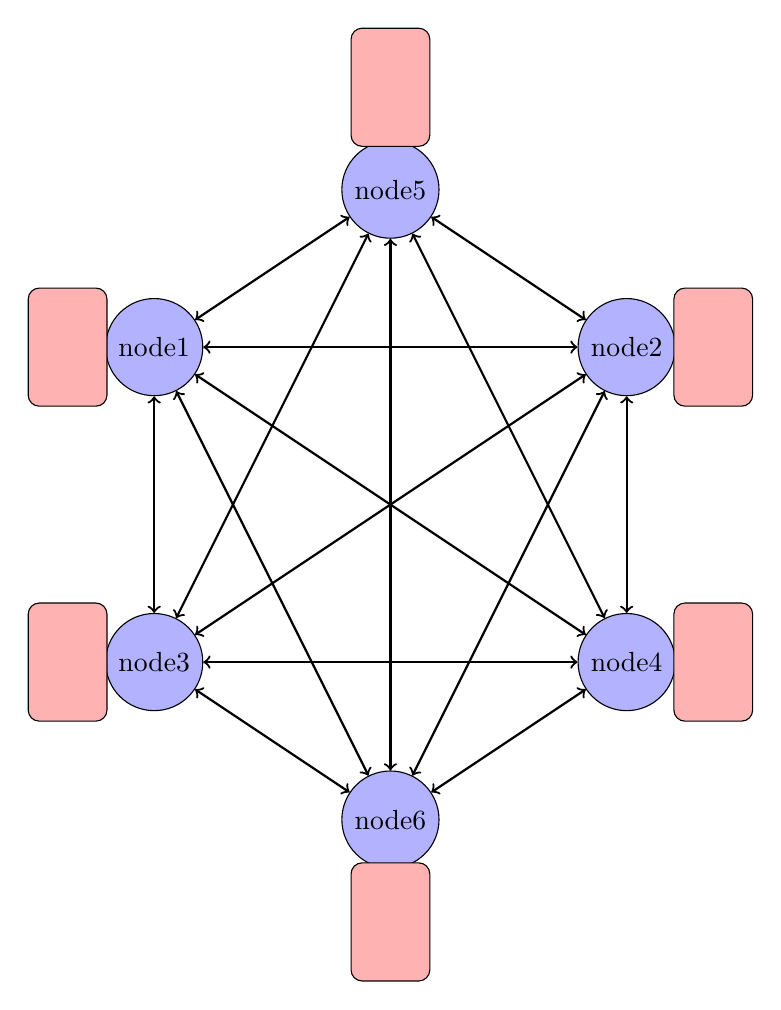
\begin{tikzpicture}[]
\node(node1)[node] {node1};
\node (pl1) [pl, left of=node1, xshift=-0.1cm] {};
\node(node2)[node, right of=node1, xshift=5cm] {node2};
\node (pl2) [pl, right of=node2, xshift=0.1cm] {};
\node(node3)[node, below of=node1, yshift=-3cm] {node3};
\node (pl3) [pl, left of=node3, xshift=-0.1cm] {};
\node(node4)[node, below of=node2, yshift=-3cm] {node4};
\node (pl4) [pl, right of=node4, xshift=0.1cm] {};
\node(node5)[node, right of=node1, xshift=2cm,yshift=2cm] {node5};
\node (pl5) [pl, above of=node5, yshift=0.3cm] {};
\node(node6)[node, right of=node3, xshift=2cm,yshift=-2cm] {node6};
\node (pl6) [pl, below of=node6, yshift=-0.3cm] {};

\draw[<->, thick] (node1) -- (node2);
\draw[<->, thick] (node1) -- (node3);
\draw[<->, thick] (node1) -- (node4);
\draw[<->, thick] (node1) -- (node5);
\draw[<->, thick] (node1) -- (node6);
\draw[<->, thick] (node2) -- (node3);
\draw[<->, thick] (node2) -- (node4);
\draw[<->, thick] (node2) -- (node5);
\draw[<->, thick] (node2) -- (node6);
\draw[<->, thick] (node3) -- (node4);
\draw[<->, thick] (node3) -- (node5);
\draw[<->, thick] (node3) -- (node6);
\draw[<->, thick] (node4) -- (node5);
\draw[<->, thick] (node4) -- (node6);
\draw[<->, thick] (node5) -- (node6);
\end{tikzpicture}


\subsection{Transactions}
Everything in crypto-currency comes under transactions, i.e. someone is sending some amount of money to someone else at some time. So a basic or overall transaction data can be structured as,

\fbox{\colorbox{lightgray}{\parbox[b][4cm][c]{0.50\linewidth}{
\textbf{\texttt{\noindent Transaction :: \{\\
\hspace*{1cm} \textless Transaction\_id\textgreater,\\
\hspace*{1cm} \textless TimeStamp\textgreater,\\
\hspace*{1cm} \textless Sender\_Id\textgreater,\\
\hspace*{1cm} \textless Receiver\_Id\textgreater,\\
\hspace*{1cm} \textless Amount\_Unit\textgreater\\
\noindent \}}}
}}}

This transaction details is send to every peer to verify. If they heard already about it, it is true, or it is false (same as women's un-manipulated gossip in village). If more than 50\% population declare it true, then it is allowed to be in the Public Ledger.

\subsection{Public Ledger}
This is the publicly shared record of transactions kept as a list of blocks. At a particular point of time everybody (every node), who are connected to the network, should have a same copy of ledger in their own devices of what server has. Whenever a new person logs into the network aotomatically the server forces to update the ledger to the person's device. So basically the ledger is the chain file.

\subsection{Chain of Blocks}
It means list of blocks of data having some common part with previous and next block. This is like Single-way linked-list(every node consists of data and program memory address to the next node). Every block contains a number of transactions and many more things.

\fbox{\colorbox{lightgray}{\parbox[b][6cm][c]{0.75\linewidth}{
\textbf{\texttt{\noindent Block :: \{\\
\hspace*{1cm} \textless Block\_Id\textgreater,\\
\hspace*{1cm} \textless TimeStamp\textgreater,\\
\hspace*{1cm} \textless Merkle\_Root\textgreater,\\
\hspace*{1cm} \textless Verifier\_Id\textgreater,\\
\hspace*{1cm} \textless Nonce\_Value\textgreater,\\
\hspace*{1cm} \textless Previous\_Hash\textgreater,\\
\hspace*{1cm} \textless Current\_Hash\textgreater,\\
\hspace*{1cm} \textless Data :: ANumberOfTransactions\textgreater\\
\noindent \}}}
}}}

So it is kind of backword linked-list which is propagating by having the previous block's kind of identity (because there is a mild chance of collision i.e. multiple values' hashes are same) hash.

\subsection{Timestamp}
The time means absolute global date-time in the format: 

\fbox{\colorbox{lightgray}{\parbox[b][2cm][c]{\linewidth}{
\textbf{\texttt{\noindent TimeStamp :: String (
\textless day\_of\_week\_code :: ddd\textgreater,
\textless month\_code :: mmm\textgreater,
\textless day\_of\_month :: dd\textgreater,
\textless year :: yyyy\textgreater,
\textless time :: hh:mm:ss\textgreater,
\textless Distance from Mean-TimeLine :: GMT+hhmm\textgreater,
\textless Time Zone :: Country\_Name Standard Time\textgreater
\noindent )}}
}}}

Example: \textbf{\q{Sat May 25 2019 20:45:04 GMT+0530 (India Standard Time)}}. The timestamp is one of the most needed to prove it later for verification of the record. It is used to create the current block's hash.

\subsection{Hash}
The job of a hash algorithm is to map any size of domain to a particular size of range. SHA-256 is one of the most popular hash algorithms which takes any length input and returns 256 bit output. All input/output operations can be transferred into strings.

\subsection{Merkle Root Hash}
Merkle tree is a complete binary tree which has the hash values of transaction data as leaf nodes. The tree propagation occures from leaves to root as tournament tree form. For any point,

			parent hash = hash(child-1 hash + child-2 hash);

A little change in any data of any transaction will change the merkle root, and thus the block's hash and the complete chain. Because it is used to create the current block's hash.

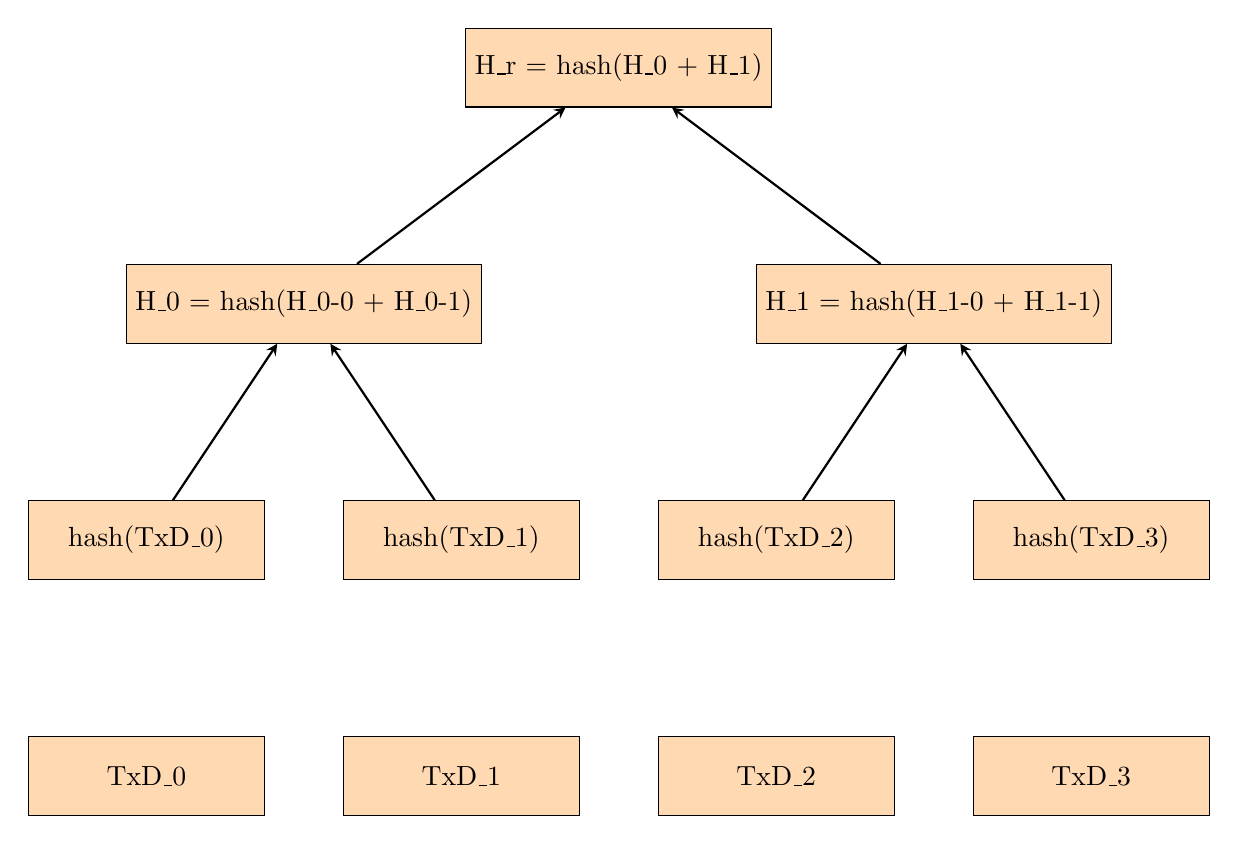
\begin{tikzpicture}[]
\node (root) [process] {H\_r = hash(H\_0 + H\_1)};
\node (child1) [process, below of=root, xshift=-4cm, yshift=-2cm]{H\_0 = hash(H\_0-0 + H\_0-1)};
\node (child2) [process, below of=root, xshift=4cm, yshift=-2cm]{H\_1 = hash(H\_1-0 + H\_1-1)};
\node (child3) [process, below of=child1, xshift=-2cm, yshift=-2cm]{hash(TxD\_0)};
\node (child4) [process, below of=child1, xshift=2cm, yshift=-2cm]{hash(TxD\_1)};
\node (child5) [process, below of=child2, xshift=-2cm, yshift=-2cm]{hash(TxD\_2)};
\node (child6) [process, below of=child2, xshift=2cm, yshift=-2cm]{hash(TxD\_3)};

\node (txd0) [process, below of=child3, yshift=-2cm] {TxD\_0};
\node (txd1) [process, below of=child4, yshift=-2cm] {TxD\_1};
\node (txd2) [process, below of=child5, yshift=-2cm] {TxD\_2};
\node (txd3) [process, below of=child6, yshift=-2cm] {TxD\_3};

\draw [arrow] (child1) -- (root);
\draw [arrow] (child2) -- (root);
\draw [arrow] (child3) -- (child1);
\draw [arrow] (child4) -- (child1);
\draw [arrow] (child5) -- (child2);
\draw [arrow] (child6) -- (child2);
\end{tikzpicture}


\subsection{Previous Hash}
The previous block's hash. It is required to maintain the chain system because we can not create the next address and we don't know when it would be created, so it is better to store what we already have. It is used to create the current block's hash.

\subsection{Nonce}
It is the quantity of computation power used to solve a mathematical problem which is not so hard but not so easy either. Too easy solution will be easy to break and too hard solution will take so long time to create a block that the adversary with huge computation power have a chance to alter the data before creating and verifying a block. Rather a medium hard problem will be better. It is used to create the current block's hash.

This is to show the verifiers that the block creator have spent sufficient amount of computation power before creating the block and also to delay the process a little bit and this is called POW (Proof of Work). In bitcoin the problem is to find the first hash of given values which is having 'd' number of leading 'zero's where the 'd' represents the difficulty of the problem i.e. the more 'd' gets it will take longer to calculate. Typical value of 'd' is 32 bits and average delay for the whole block addition (create, verify then add) is about 10 minutes.

\subsection{Consensus Mechanism}
It is the contract or the protocol by which the blocks are verified and the winning blocks are added to everyone's ledger as well as the central server. The actual consensus algorithm is not published for security reasons. But by possible ways or reverse eengineering people have created  different models. Some of those models are:

\begin{figure}
\begin{center}
\includegraphics[width=0.75\textwidth]{./img_src/bitcoin.jpg}
\end{center}
\caption{Overview of BitCoin Technology (BCTs).}
\end{figure}

\begin{enumerate}
\item Probable bitcoin consensus mechanism
\item Paxos (Part-Time Parliament) consensus mechanism~\cite{paxos_made_easy, paxos_made_practical}
\item Raft consensus mechanism~\cite{raft_extd}
\end{enumerate}

Bitcoins one is probably the simplest one, but having bugs. The Paxos allows different types of sources and faults to come, it learns and fixes it. Raft does not allow any fault to happen.

The basic overall way in which consensus happen in bitcoin might be the following,

\begin{enumerate}
\item The transaction comes to server from client nodes;
\item Server stores that in file system database as unverified transaction;
\item At the point of interval of 10 minutes server broadcasts it to the miners network i.e. to every miner;
\item Each miner individually verifies and adds correct transaction in a block. Each node holds its block creation and validates the new block as soon as it gets new block from network. Who's block is valid and introduced first to network will be added to everyone's chain and they will start making new block on top of it. Sometimes forks might be created for the networking distance between distant nodes, at that moment conflict will come. If a new introduced block's previous hash does not match with the last block's current hash the node requests to the network to get the missing blocks one by one until the blocks match, it validates it, delete the wrong blocks (make them orphan) and add missing blocks to own chain to resolve fork and maintain longest updated chain. So it is a race between miner nodes.
\item Server gets a copy from miners group and updates own copy and delete the added tansactions from file system.
\end{enumerate}

\subsection{Applications of BCTs}
Block-Chain Technology provides one major advantage over conventional centralized database system: immunity from unexpected data changes or Hacks, which gives rise to numerous applications. Some of them include

\begin{itemize}
\item Crypto-currency: Creating and transferring digital money, Data Mining.
\item Military applications: Secure and verified records of Every Military Events and documents.
\item Structural health Monitoring
\item e-Biding Systems
\item Election System or e-Voting Systems
\item Selling Records and other Commercial Applications
\item Music Copyright Verification System
\item Integrity Analysis of Media Files
\end{itemize}

\subsection{Application}
Some of the commercial applications built on blockchain technology are as follows,

\subsubsection{BitCoin}
One year after creating protocols of BlockChian for cryptocurrency, Satoshi Nakamoto in 2009 released the first source code for BitCoin (BTC) application. Bitcoin has since grown rapidly to a market footprint of around 39 billion U.S. dollars (as of 12 Jul 2017). BTC is a decentralized cryptocurrency using a permissionless blockchain that every user has the ability to download and thereby check. The users of the network use their personal computational power to verify transactions through hashes, i.e., mining. The total computational power of the Bitcoin network is estimated to be more than 256 times the power of the world's 500 top supercomputers.
Site: \href{https://bitcoin.org/}{BitCoin}.

\subsubsection{HyperLedger}
Hyperledger is a project under the Linux Foundation which seeks to provide a unified blockchain architecture for industrial applications. Hyperledger is a collaboration of more than 100 organizations focused on banking, supply chain, and other transaction networks. It uses BFT system to reach consensus by fewer number of nodes.
\href{https://www.hyperledger.org/}{HyperLedger}

\subsubsection{Ethereum}
It is a permissionless blockchain made as a smart contracts platform run by Ether (ETH). The verification is done through the peer to peer network which constitutes Ethereum together with ETH which fuels the network, the consensus algorithm to share the state of the network, and the Turing complete scripting language which enables users to write complex scripts (smart contracts). It is the consensus engine which sets the speed of the Ethereum network by updating the state of the network at specific time intervals (shorter than for the Bitcoin network). The Ethereum network is fueled by gas which is a unit connected to ETH which is used to pay for the storage and computations an application (smart contract) needs.
\href{https://www.ethereum.org/}{Ethereum}

Solidity is a programing language build specifically to target the Ethereum virtual Machine (EVM) which in turn is the protocol to access the blockchain. Solidity has a syntax similar to JavaScript and is the language in which many smart contracts are written. The smart contracts are then compiled into bytecode and fed into to EVM and thus they can operate on the blockchain. In Ethereum are every transaction and smart contract is saved on the blockchain. The blockchain is in turn distributed and the states are handled by the consensus algorithm.
\href{https://solidity.readthedocs.io/en/v0.5.7/}{Solidity}

\subsubsection{Tendermint}
Tendermint is not a blockchain in itself but rather a general purpose blockchain consensus engine with a consensus layer for blockchaining. Tendermint can be used as a replacement for the consensus engines of other blockchains. It runs BFT algorithm.
\href{https://tendermint.com/}{Tendermint}

\subsubsection{Eris:db}
Eris:db is a controllable (permissible), smart contract-enabled, PoS based blockchain design with the PoS based on Tendermint. Eris:db is an application layer for blockchain applications. Eris is the backbone for deploying and interacting with the application logic.
\href{https://github.com/vulcanize/eris-db}{Eris:db}

\subsubsection{Cumulus}
Cumulus is a blockchain solution developed by Ericsson. Cumulus builds on and works with the Ethereum Virtual Machine (EVM) but separates the consensus algorithm and the blockchain from the EVM. Cumulus works similar to Ethereum; however, it is a private blockchain which means it does not run on gas.
\href{https://github.com/ubclaunchpad/cumulus}{Cumulus}

\subsection{Comparison}
There are a number of blockchain solutions to choose from, some of the most important ones are described in the previous subsections. For this thesis we will use a hybrid one, that supplies our requirements or logical proposal.

\begin{center}
\begin{tabular}{|c|c|c|c|c|c|}
\hline
\textbf{Name} & \textbf{Distribution} & \textbf{Transactions/second} & \textbf{Consensus Algorithm} \\
\hline
\textbf{Hyperledger} & Private & 10k & BFT \\
\hline
\textbf{Eris:db} & Private & 10k & Tendermint(PoS) \\
\hline
\textbf{Ethereum} & Public & 20 & PoS \\
\hline
\textbf{Tendermint} & Private & 10k & Tendermint BFT \\
\hline
\textbf{Bitcoin} & Public & 7 & PoW \\
\hline
\textbf{Cumulus} & Private & (untested) & (unknown) \\
\hline
\end{tabular}
\end{center}

\subsection{Security and Integrity in BCTs}
As the data is not sitting on a single data server so there is no security issue for Server Hacking. And also the hash-Chain with Cryptography makes it near to impossible to figure out or change previous data block in the blockchain. Before adding any data block with the help of consensus mechanism the blocks are verified with the digital signature of the node and some solution of nonce (the number of times the cllient application required to calculate the mathematical problem) and various other meta data.
As in some interval the system is refreshing itself, if some error seems to be occured, it backs up itself by contacting the miners (the trusted nodes), compare their files and back up with the valid one. So no integrity problem is there, unless and until the internet works fine.


\section{Machine Learning}
\label{sec:mlearning}
% Machine Learning
A machine is said to be learning from past Experiences(data feed in) with respect to some class of Tasks, if it's Performance in a given Task improves with the Experience.

According to a famous person, Machine Learning is a system that can learn from example through self-improvement and without being explicitly coded by programmer. The breakthrough comes with the idea that a machine can singularly learn from the data (\textit{i.e.} media database of real life objects, numbers dataset from algorithms, face images, job dtabase) to produce accurate results.

Machine learning combines data with statistical tools to predict an output. This output is then used by corporate to makes actionable insights. Machine learning is closely related to data mining and Bayesian predictive modeling. The machine receives data as input, use an algorithm to formulate answers.

A typical machine learning tasks are to provide a recommendation. For those who have a Netflix account, all recommendations of movies or series are based on the user's historical data. Tech companies are using unsupervised learning to improve the user experience with personalizing recommendation.

\subsection{Machine Learning vs. Traditional Programming}
Traditional programming differs significantly from machine learning. In traditional programming, a programmer code all the rules in consultation with an expert in the industry for which software is being developed. Each rule is based on a logical foundation; the machine will execute an output following the logical statement. When the system grows complex, more rules need to be written. It can quickly become unsustainable to maintain.

Machine learning is supposed to overcome this issue. The machine learns how the input and output data are correlated and it writes a rule. The programmers do not need to write new rules each time there is new data. The algorithms adapt in response to new data and experiences to improve efficacy over time.

\subsection{How does Machine learning work}
Machine learning is the virtual brain where all the learning takes place. The way the machine learns is similar to the human being. Humans learn from experience. The more we know, the more easily we can predict. By analogy, when we face an unknown situation, the likelihood of success is lower than the known situation. Machines are trained the same. To make an accurate prediction, the machine sees an example. When we give the machine a similar example, it can figure out the outcome. However, like a human, if its feed a previously unseen example, the machine has difficulties to predict.

The core objective of machine learning is the learning and inference. First of all, the machine learns through the discovery of patterns. This discovery is made thanks to the data. One crucial part of the data scientist is to choose carefully which data to provide to the machine. The list of attributes used to solve a problem is called a feature vector. You can think of a feature vector as a subset of data that is used to tackle a problem.

The machine uses some fancy algorithms to simplify the reality and transform this discovery into a model. Therefore, the learning stage is used to describe the data and summarize it into a model.

For instance, the machine is trying to understand the relationship between the wage of an individual and the likelihood to go to a fancy restaurant. It turns out the machine finds a positive relationship between wage and going to a high-end restaurant: This is the model

\subsubsection{Inferring}
When the model is built, it is possible to test how powerful it is on never-seen-before data. The new data are transformed into a features vector, go through the model and give a prediction. This is all the beautiful part of machine learning. There is no need to update the rules or train again the model. You can use the model previously trained to make inference on new data.

The life of Machine Learning programs is straightforward and can be summarized in the following points:
\begin{enumerate}
\item Define a question
\item Collect data
\item Visualize data
\item Train algorithm
\item Test the Algorithm
\item Collect feedback
\item Refine the algorithm
\item Loop 4-7 until the results are satisfying
\item Use the model to make a prediction
\end{enumerate}

There are two main types of Learning,
\subsubsection{Supervised learning}
An algorithm uses training data and feedback from humans to learn the relationship of given inputs to a given output. For instance, a practitioner can use marketing expense and weather forecast as input data to predict the sales of cans.

You can use supervised learning when the output data is known. The algorithm will predict new data.

There are two categories of supervised learning:
\paragraph{Classification}
Imagine you want to predict the gender of a customer for a commercial. You will start gathering data on the height, weight, job, salary, purchasing basket, etc. from your customer database. You know the gender of each of your customer, it can only be male or female. The objective of the classifier will be to assign a probability of being a male or a female (\textit{i.e.}, the label) based on the information (\textit{i.e.}, features you have collected). When the model learned how to recognize male or female, you can use new data to make a prediction. For instance, you just got new information from an unknown customer, and you want to know if it is a male or female. If the classifier predicts male = 70\%, it means the algorithm is sure at 70\% that this customer is a male, and 30\% it is a female.

The label can be of two or more classes. The above example has only two classes, but if a classifier needs to predict object, it has dozens of classes (\textit{e.g.} glass, table, shoes, etc. each object represents a class).

\paragraph{Regression}
When the output is a continuous value, the task is a regression. For instance, a financial analyst may need to forecast the value of a stock based on a range of feature like equity, previous stock performances, macroeconomics index. The system will be trained to estimate the price of the stocks with the lowest possible error.

\subsubsection{Unsupervised learning}
In unsupervised learning, an algorithm explores input data without being given an explicit output variable (\textit{e.g.} explores customer demographic data to identify patterns)

You can use it when you do not know how to classify the data, and you want the algorithm to find patterns and classify the data for you

Challenges and Limitations of Machine learning
The primary challenge of machine learning is the lack of data or the diversity in the dataset. A machine cannot learn if there is no data available. Besides, a dataset with a lack of diversity gives the machine a hard time. A machine needs to have heterogeneity to learn meaningful insight. It is rare that an algorithm can extract information when there are no or few variations. It is recommended to have at least 20 observations per group to help the machine learn. This constraint leads to poor evaluation and prediction.

\subsection{Application}
There are plenty of application fields where ML is being used for better performance,
\subsubsection{Augmentation}
Machine learning, which assists humans with their day-to-day tasks, personally or commercially without having complete control of the output. Such machine learning is used in different ways such as Virtual Assistant, Data analysis, software solutions. The primary user is to reduce errors due to human bias.
\subsubsection{Automation}
Machine learning, which works entirely autonomously in any field without the need for any human intervention. For example, robots performing the essential process steps in manufacturing plants.
\subsubsection{Finance Industry}
Machine learning is growing in popularity in the finance industry. Banks are mainly using ML to find patterns inside the data but also to prevent fraud.
\subsubsection{Government organization}
The government makes use of ML to manage public safety and utilities. Take the example of China with the massive face recognition. The government uses Artificial intelligence to prevent jaywalker.
\subsubsection{Healthcare industry}
Healthcare was one of the first industry to use machine learning with image detection.
\subsubsection{Marketing}
Broad use of AI is done in marketing thanks to abundant access to data. Before the age of mass data, researchers develop advanced mathematical tools like Bayesian analysis to estimate the value of a customer. With the boom of data, marketing department relies on AI to optimize the customer relationship and marketing campaign.
\subsubsection{Supply Chain}
Machine learning gives terrific results for visual pattern recognition, opening up many potential applications in physical inspection and maintenance across the entire supply chain network.

Unsupervised learning can quickly search for comparable patterns in the diverse dataset. In turn, the machine can perform quality inspection throughout the logistics hub, shipment with damage and wear.

For instance, IBM's Watson platform can determine shipping container damage. Watson combines visual and systems-based data to track, report and make recommendations in real-time.

In past year stock manager relies extensively on the primary method to evaluate and forecast the inventory. When combining big data and machine learning, better forecasting techniques have been implemented (an improvement of 20 to 30 \% over traditional forecasting tools). In term of sales, it means an increase of 2 to 3 \% due to the potential reduction in inventory costs.

\paragraph{Google Car}
For example, everybody knows the Google car \textbf{Waymo}. The car is full of lasers on the roof which are telling it where it is regarding the surrounding area. It has radar in the front, which is informing the car of the speed and motion of all the cars around it. It uses all of that data to figure out not only how to drive the car but also to figure out and predict what potential drivers around the car are going to do. What's impressive is that the car is processing almost a gigabyte a second of data.


For our case we use logistic regression (discussed in Appendix app:4) and the algorithm is discussed in Proposal chapter \ref{ch:3}.


\section{Security}
\label{sec:security}
In this thesis project data integrity is of paramount importance. In order to be able to trust the data stored within the blockchain, a reliable secure connection is created between the application running on cleent's device and the computer that is computing the blockchain. User side application collects the data and creates the consecutive transaction which is to be sent between the device and the server where the blockchain computations are done, therefore it is impossible for a third party to know what the plaintext representation of the image is.
As a result encryption of this transaction might be of less importance. However, it is crucial for the system to know that the integrity of the hash is intact. The image captured and stored at a device can later be verified as to what is received by another device by using the blockchain.
An HTTP connection is used between the device and the server. The HTTP connection will in future implementation be replaced with a HTTPS connection to secure the communication.

\begin{figure}
\begin{center}
\includegraphics[width=\textwidth]{./img_src/client_server.png}
\end{center}
\label{fig_connClientServer}
\caption{A secure connection between Client and Server}
\end{figure}

\section{Client Side}
\label{sec:client}
A client may have a smartphone (of the brand Android, iPhone) or a computer (laptop or desktop). All of these devices comes with a default web-browsing tool like Google Chrome, Microsoft Edge, Mozilla Firefox or Mac Safari etc. All else a client needs an active reliable internet connection to communicate with sever. Moreover the miners have to have computers with better computation power. With the advancement of web programming languages with lots of APIs now it is very easy to capture an image or handle a local file and pass the data to the peer-to-peer network.

\subsection{JavaScript}
In this thesis, basic js is used as the run-time environment together with the inbuilt JS library installed on the browser. We are trying to use Node.js (also along with our code) that runs there servers, i.e., the consensus server. Note that all three servers run within the node.js environment on the computer hosting the web server and blockchain. JavaScript is the front end development language which realizes the functionality of the web page. JavaScript works together with PHP (HTML in it) and CSS in order to deliver a nice looking functional web page.

\section{Server Side}
\label{sec:server}
\subsubsection{PHP Server}
The Server side is made of PHP (HTML-5). In order to easy communicate with the blockchain from both the client device and the server running the verification client PHP APIs used over the HTTP protocol, usually to the server's TCP port 80. An apache server is basically a web server architecture which enables clients to make a request of servers. The HTTP protocol builds upon a request/response relationship between a client and a server and in this case used within the LAMPP architecture. In HTTP a string is sent to a specific port on the server with a specific method predefined by the HTTP standard. The most common methods are: GET, HEAD, POST, and PUT. The POST method is used by both the Android device and the web client of this thesis project to give both the ability to add and via the reply to this POST request to get information from the server. The communication between JS and PHP is done with XML-HTTP request with JSON byte stream. There is every type of handwriten PHP code to handle any type of request to Server.
\subsubsection{POST Method}
The POST method is a standard method in the HTTP protocol and gives the user the ability to add and receive data from the server. A HTTP transaction session is established through a TCP connection to a specific port on the server. After the TCP connection is established, of plain text HTTP message is sent to the other who either confirms the transaction or responds with an error message. It is in the body of this message that the response to the sender will be sent. Within the scope of this thesis the response will either be a boolean variable showing a successful transmission or a string of hashes requested from the blockchain.
\subsubsection{HTTPS}
Hypertext Transfer Protocol Secure (HTTPS) is an encrypted version of the HTTP protocol. HTTPS is usually used for sensitive information such as banking, private information, or classified information. HTTPS usually uses port 443 rather than HTTP port 80. In order for a user to be able to trust that a server is who it says that it issigned, third party certificates are used, usually in conjuction with the use of the Secure Socket Layer (SSL) as a secure transport protocol. A third party provides the server with a signed certificate which the user of the service verifies. Now that the user has verified the identity of the client and the server has verified the identity of the client - and encryption between the two parties may be set up. The security depends on that the certification chain work, that the user knows which server to use and that the user (client) notices when the certificate is incorrect or missing. Furthermore, in order to provide a high level of security the keys and the algorithms used need to be strong.

\section{Related Works}
\label{sec:prevWorks}
\subsection{Old possible works}
The process of image integrity checking is old job and many algorithms have been made. The following is the overview of them.
\begin{enumerate}
\item Store the real images in some database. Match the testing image with the existing one bit by bit.
\item Like in previous case, store it and check the new one's hash with the existing one's hash.
\item Searching the image in different databases using object detection and context similarity.
\item Every digital image is created in an electronic device which is having some unique property or signature in the world. The softwares that has created the image are designed in such a way that they put the digital signature in the metadata field of the image, let's say EXIF data for JPEG images. Any software that knows the byte signatures can detect the random image is original or not by checking the signature and named context that lies inside of the image file.
\item By checking the image context with reality or possiblity, some images can be checked.
\item An expert or hacker not only seeks for the context or visual similarity, but an expert knows that secret figures (WaterMarking) secret messages (Steganography) can be embedded in the image file, because the main image is a 2d matrix of intensity values (list of integers for BnW, RGBA, CMYK, or other) at different pixel positions.
\item The modern approach is to use deep neural network that learns and tries to detect image integrity in about 90\% efficiency and accuracy.
\item Image Forensics uses about all of the previous ones.
\end{enumerate}

\subsection{Related Work}
This section presents related work done both in the academic world and the industry.
\subsubsection{Academic}
Three different academic papers have been identified as relevant to this research. The following subsections highlight their main points and relevance to this thesis project.
\paragraph{Timestamping video footage in traffic incidents}
In ~\cite{gkb_bitcoin} Gipp, Krosti, and, Breitinger investigated the use of the Bitcoin network to timestamp a video feed from a smartphone camera placed in a car in the event of an accident.
\paragraph{Trusted Timestamping}
With regards to trusted timestamping two reports were identified: \q{Trusted Timestamping} ~\cite{gmg_bitcoin} and \q{Commitcoin} ~\cite{ce_commitcoin}. Both solutions leverage the time stamp made using the Bitcoin protocol when creating a transaction together with the carbon dating nature of the blockchain (i.e., one can tell the rough date of an entry by looking at the sequence of time stamps). These two solutions are slightly different in terms of their execution, but the basic theory of using the existing Bitcoin blockchain is the same.
\paragraph{Forensics Investigations of Multimedia Data}
In ~\cite{pt_forensics}, R. Poisel and S. Tjoa review the latest trends in forensic investigations of multimedia data, i.e. images, videos, and audio files. They describe different methods for determining what has been done to images and expose fabrications down to which details within a picture have been tampered with.
\paragraph{Digital Watermarking}
I. Echizen, et al. ~\cite{esytth_watermark} insert digital watermarks into video files to detect data tampering. They begin by breaking a video file into its composonents: the video, the audio, the timecodes, and the eader. The header is used together with the timecodes to separately watermark the audio and video.
\subsubsection{Industrial}
Three different industry solutions have been identified as being relevant. The following subsections highlight their main points and relevance to this thesis project.
\paragraph{Nexan - Assureon Archive Storage}
In Assureon Archive Storage ~\cite{n_assureon} fingerprints are created from the data in order to prove the integrity of files within a data archive system. The original files are stored on at least two different disks or at two different geographical locations.
\paragraph{Enigio - time:beat}
The product series \q{time:beat} ~\cite{asa_enigio} includes: time:shot, time:stamp, time:grab, and time:mail: by Enigio. It uses to archive time stamped fingerprints of integrity sensitive materials: email, pictures, documents, and websites in a permissioned blockchain controlled and owned by Enigio.
\paragraph{Ascribe}
Ascribe ~\cite{h_intellect} helps artists to create a digital copy of their work and time-stamp it in the Bitcoin blockchain. When a file is uploaded, Ascribe creates a digital certificate which can be traded, tracked, or loaned via the blockchain using SPOOL ~\cite{dt_spool}.

\subsection{Curent Works}:
\begin{enumerate}
\item There are plenty of image storing and searching by image in the websites. In the list \href{https://images.google.com/}{Google Image}, \href{https://www.yandex.com/images/}{Yandex Images} they use the image searching by name, context.
\item Some of them uses object detection \href{https://images.google.com/}{Google Images}, \href{https://www.imageidentify.com/}{Wolfram Images}.
\item Some website programs use reverse image search like \href{https://images.google.com/}{Google Images}, \href{https://tineye.com/}{Reverse Image Search}.
\item There are plenty of softwares like the photo eding softwares itself like Photoshop, GNU Image Manipulation Program, and other editors.
\item In ~\cite{img_cnn} they used CNN for image comparing and many other that can be mentioned for well known face recognition problem.
\item In ~\cite{adam_fabian} they used a mechanism for video integrity analysis.
\end{enumerate}

\section{Summary}
\label{sec:summary}
The different parts and aspects of the proof of concept prototype were broken down and analyzed. From the smallest components of the blockchain consensus algorithms, to which existing blockchain platform should be utilized. It also talked about the ways of communication between server and client.

%\chapter{Details}
\label{Ch3}
%\setcounter{page}{1}
%\pagenumbering{arabic}
\bigskip

The process underlying the block-chain technology are the folowing:
\begin{itemize}
\item Creating Account and Be a Part of the Network with an hash id
\item Creating own Data block
\item Request the BCT System to add it by sending it to the open Network in secure or enCrypted way
\item The system then send the block to other nodes for verification
\item The other nodes can verify it with solving some nonce and report to system
\item After being verified the System will add the new block to the chain and update it to every peer's copy of the hyper-ledger
\item Data mining is useful when to check again and again for the integrity of data and the performance of the system
\end{itemize}

The following is the overview of the BitCoin implemention using concepts of blockchain,

\section{Transaction}
We define a block data masked with chain of digital signatures. Each owner transfers the coin to the
next by digitally signing a hash of the previous transaction and the public key of the next owner
and adding these to the end of the coin. A payee can verify the signatures to verify the chain of
ownership.

\section{Timestamp}
The solution we propose begins with a timestamp server. A timestamp server works by taking a
hash of a block of items to be timestamped and widely publishing the hash, such as in a
newspaper or Usenet post [2-5]. The timestamp proves that the data must have existed at the
time, obviously, in order to get into the hash. Each timestamp includes the previous timestamp in
its hash, forming a chain, with each additional timestamp reinforcing the ones before it.

\section{Proof of Work}
To implement a distributed timestamp server on a peer-to-peer basis, we will need to use a proof-
of-work system. The proof-of-work involves scanning for a value that when hashed, such as with SHA-256, the
hash begins with a number of zero bits. The average work required is exponential in the number
of zero bits required and can be verified by executing a single hash.
For our timestamp network, we implement the proof-of-work by incrementing a nonce in the
block until a value is found that gives the block's hash the required zero bits. Once the CPU
effort has been expended to make it satisfy the proof-of-work, the block cannot be changed
without redoing the work. As later blocks are chained after it, the work to change the block
would include redoing all the blocks after it.

\section{Network}
The steps to run the network are as follows:
\begin{enumerate}
\item New transactions are broadcast to all nodes.
\item Each node collects new transactions into a block.
\item Each node works on finding a difficult proof-of-work for its block.
\item When a node finds a proof-of-work, it broadcasts the block to all nodes.
\item Nodes accept the block only if all transactions in it are valid and not already spent.
\item Nodes express their acceptance of the block by working on creating the next block in the chain, using the hash of the accepted block as the previous hash.
\end{enumerate}

\section{Incentive}
By convention, the first transaction in a block is a special transaction (the block is called genesis block) that starts a new block owned
by the creator of the block. This adds an incentive for nodes to support the network, and provides
a way to initially distribute coins into circulation, since there is no central authority to issue them.
The steady addition of a constant of amount of new coins is analogous to gold miners expending
resources to add gold to circulation. In our case, it is CPU time and electricity that is expended.

\section{Claiming Memory}
Once the latest transaction in a coin is buried under enough blocks, the spent transactions before
it can be discarded to save disk space. To facilitate this without breaking the block's hash,
transactions are hashed in a Merkle Tree, with only the root included in the block's hash.
Old blocks can then be compacted by stubbing off branches of the tree. The interior hashes do
not need to be stored.

\section{Simplified Video Verification}
It is possible to verify video without running a full network node. A user only needs to keep
a copy of the block headers of the longest proof-of-work chain, which he/she can get by querying
network nodes until he's/she's convinced he/she has the longest chain, and obtain the Merkle branch
linking the transaction to the block it's timestamped in. He can't check the transaction for
himself, but by linking it to a place in the chain, he can see that a network node has accepted it,
and blocks added after it further confirm the network has accepted it.

\section{Privacy}
The traditional banking model achieves a level of privacy by limiting access to information to the
parties involved and the trusted third party. The necessity to announce all transactions publicly
precludes this method, but privacy can still be maintained by breaking the flow of information in
another place: by keeping public keys anonymous. The public can see that someone is sending
an amount to someone else, but without information linking the transaction to anyone. This is
similar to the level of information released by stock exchanges, where the time and size of
individual trades, the "tape", is made public, but without telling who the parties were.

\chapter{Proposal}
\label{ch:3}
\bigskip

Using the concepts of Block-Chain we propose our algoorithms for Image Integrity Analysis D-APP system.

We are trying to build a web-based social media application like WhatsApp and that will be connected with the online server running blockchain in it. The process of verification of the media (text, image or video) for checking fakeness or scam in a nutshell will be as follows,

As mentioned earlier, the main jobs of our project to build a small social media platform that will store images, show them in news feed and not only that, someone can bring an image and perform search operation in the system to check if we know about the image or not, i.e. if the image is valid or not.

The system we are proposing is a hybrid of previous strict systems in terms of Permission (Permissioned/Non-permisionalized) and Centralization (Centralized/Decentralized) along with some extra mechanisms. And also we preserve the scalability of the implementation that it is not necessary to have a dedicated huge computation power for all.

\section{Workflow}
The following is the control flow of the overall processes,
\begin{enumerate}
\item An user will have to log into the system first to be a part of the system;
\item There are two types of users, some are normal users and rest are miners who have some extra powers as well as responsibilities.
\item Normal users are those who will come to share their images by upload or taken from their camera interface and also search images for checking. In their home page they can scroll and click an image for viewing, search signatures, download images to own devices.
\item The miners are the creators of the blocks i.e. they will have computation power to generate the blocks, store the blocks in their own computers and broadcast them in the miners network, gossip among each others. They verify transactions before putting into a block.
\end{enumerate}

\section{System Design}
In one side of the system, the normal user can request the system either to store an image or to verify. On storing request the server will help the client's device to resize the image in a particular dimention (image preprocessing) and generate the correct request format in terms of transaction (Tx). Then the server will create a copy of it making a symmetric key encryption over assymetric key encryption of the user and store in own file system database in unverified or new transaction file.

On a certain time interval (not so long, not so small, bitcoin takes 10 minutes, we will take it 5 minutes) the miners will be verifying these pool of unverified transactions and adding them in new blocks in parallel through consensus mechanism. Our consensus mechanism works as follows,

\begin{figure}
\begin{center}
\includegraphics[width=0.75\textwidth]{./img_src/blockchain_network.jpg}
\end{center}
\caption{Consensus mechanism}
\end{figure}

\subsection{Consensus mechanism}
\begin{enumerate}
\item At a time interval the server will broadcast the transactions or the miners will get them on request from the server database through XML-HTTP or SFTP protocol.
\item The miners either individually or by gossiping will verify the transaction data. Verifying by own will create the uniqueness, by gossiping maintains the correctness that prevent the fault from any side (server, other miners, itself).
\item After they delete the invalid transaction set they will start creating new block out of it.
\item After a node discovers or completes creating a new block, it broadcasts to the miner network and waits for confirmation and others blocks. After a node gets a new block, it holds it's own computation and validate the new block. If the new block is valid and the node have all previous blocks that should be linked in the chain by previous hash the node keeps it into own temporary space, and wait for others for confirmation, and if not valid then resume own computation. After all blocks say we have a valid block (either own or someone else's) to each other, they compare with what other nodes are having. The winner is one of the blocks which is having most of the criterias below,
\begin{enumerate}
\item Biggest in size $\implies$ It is having maximum number of transactions
\item Bigger nonce $\implies$ Most computation power is spent for it.
\item Lowest rewarded miner $\implies$ To remove partiality and create balance and good understanding between miners.
\end{enumerate}
After 5 minutes the server requests the miners to get the decided block to be added in the chain. Server validates the block and adds it in the chain and remove the transactions that are either added or marked as invalid from the transaction pool.

\begin{figure}
\begin{center}
\includegraphics[width=0.75\textwidth]{./img_src/block_chain.png}
\end{center}
\caption{Block Creation}
\end{figure}

\item On request of an image verification, first the image metadata is being checked (1st phase). If the metadata contains the our system generated signature, it will decrypt it and check in that particular block or the range of the blocks for the transaction that contains the image as well as the user's profile for it. Becacuse while creating downloadable file the system encrypts and adds the metadata in the image file. If found, it generates the confirmation message and the links regarding it. And if not then the system requests for time and search the entire blockchain database for hashes (2nd phase). If found it does the same. And still if it not found, it runs a deep CNN for searching for contexts or by object for maximum possible proof (3rd phase). The result it gives now is the final result.
\item The process continues again and again recursively.
\end{enumerate}

\section{Image Comparison Scheme}
The following diagram shows how all the 3 steps the system should follow to chech if an image is already in the system or not \textit{i.e.} Signature Match, Hash Match, Context Match.

The image comparison technique we are trying to build at 3rd level of verification is as follows.
Comparing the two images byte by byte, if the difference between two images is less then the threshold value then image will be same, otherwise we consider that comparison as -(ve) result. To decide the value of threshold we will use machine learning, in which we train our system to decide the threshold value.

\begin{enumerate}
\item We will \q{Get Uploaded Bytes} (GUB) from the file using file uploader api of HTML-5;
\item Then we will try to \q{Extract Metadata} and Search for digital signatures that is expexted to be generated and included by our system;
\item Checking if \q{Signature Found} is true go to 4, else go to 9;
\item Process Signature to get Blocks and Transaction metadata, \textit{i.e.} \textbf{who}, \textbf{where}, \textbf{when} created \textbf{what}.
\item \q{Match Current Metadata with Transactions} (MCMwT) in that Block.
\item If \q{Is Match Found} gives No do nothing, else go for 2nd level matching (next step).
\item \q{Generate Hash} from the image and \q{Match Hash} between the narrowed down two images.
\item If \q{Are Equal} gives true then the Exact match has found, else go for level-3 verification for the two images (discussed in previous paragraph).
\item \q{Generate Hash} for 2nd level verification.
\item \q{Match in All Transactions in All Blocks} for the hash.
\item If \q{Is Found} gives Yes that means an exact match found, else go for level-3 verification for context \q{Match in All Transactions in All Blocks} and it will take a huge amount of time.
\end{enumerate}

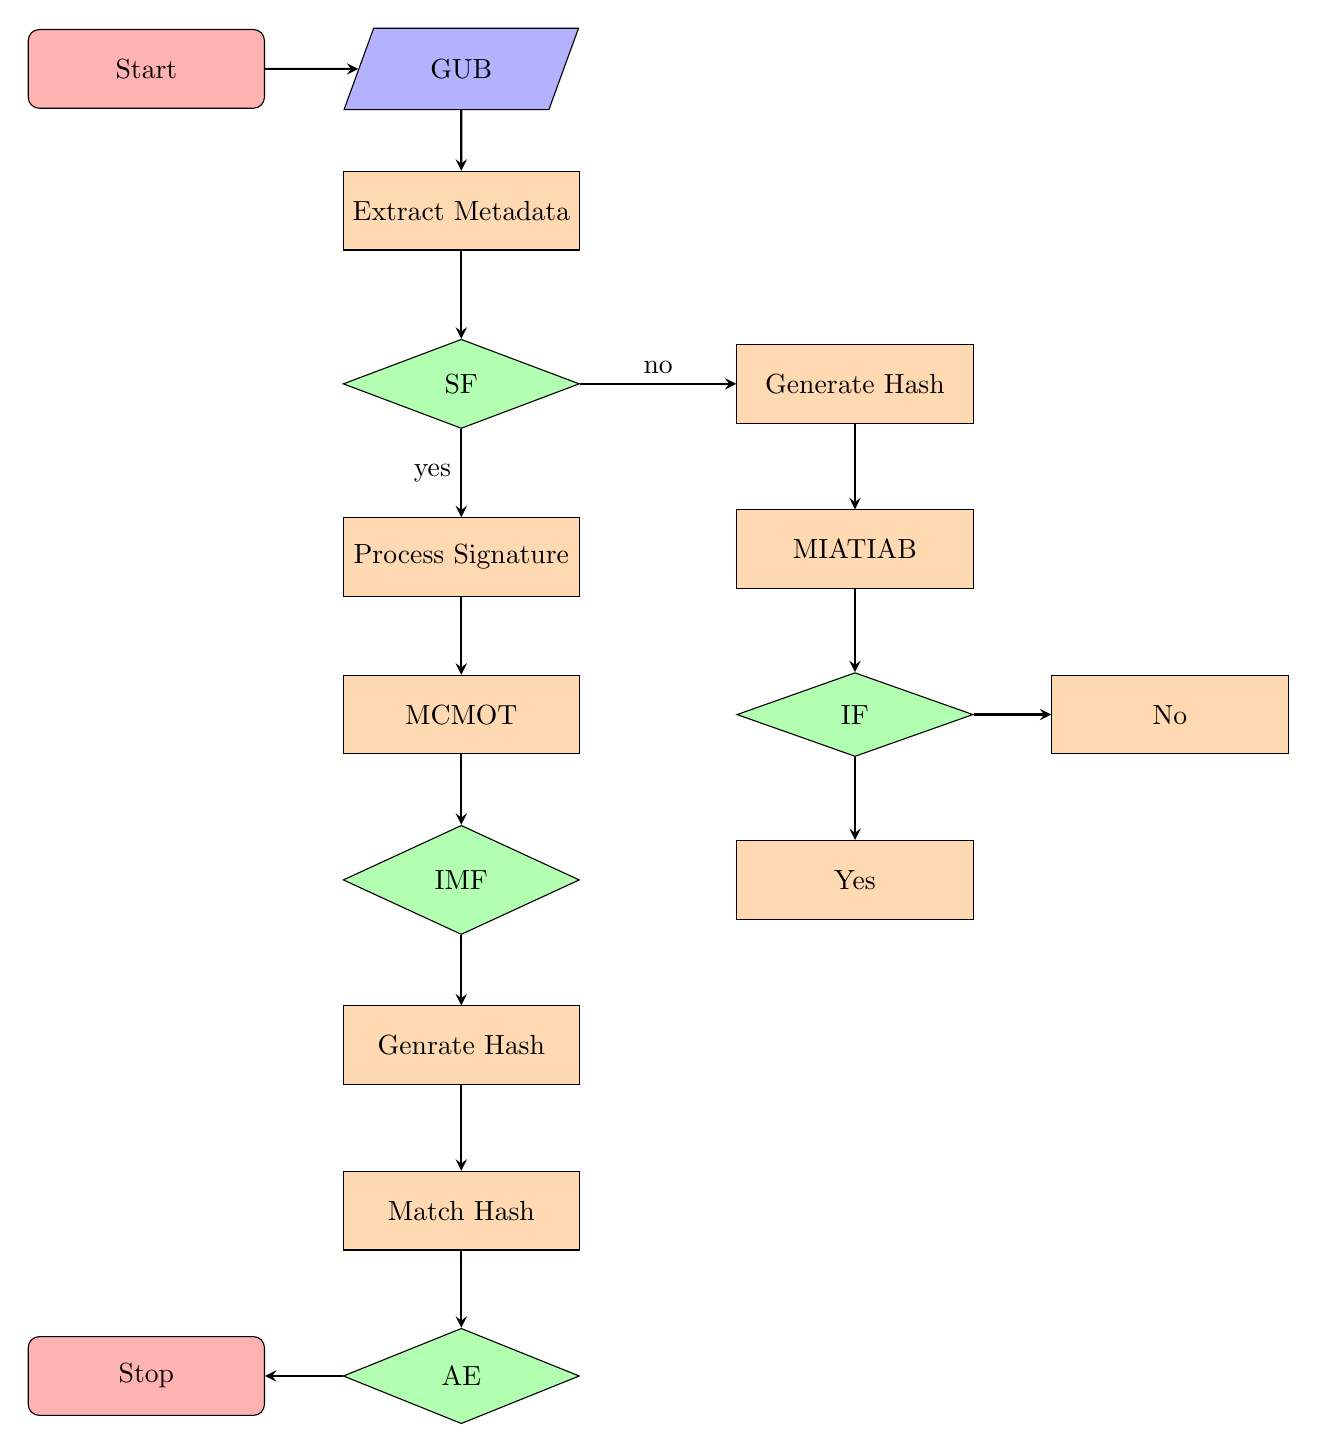
\begin{tikzpicture}[node distance=2cm]
\node (start) [startstop] {Start};
\node (in1) [io, right of=start, xshift=2cm] {GUB};
\node (pro1) [process, below of=in1,yshift=0.2cm] {Extract Metadata};
\node (dec1) [decision, below of=pro1, yshift=-0.2cm] {SF};
\node (pro2a) [process, below of=dec1, yshift=-0.2cm] {Process Signature};
\node (pro2b) [process, right of=dec1, xshift=3cm] {Generate Hash};
\node (out1) [process, below of=pro2a] {MCMOT};
\node (check2) [decision,below of=out1,yshift=-0.1cm]{IMF};
\node (ghash) [process, below of=check2,yshift =-0.1cm] {Genrate Hash};
\node (mhash) [process, below of=ghash,yshift = -0.1cm]{Match Hash};
\node (ismhash) [decision, below of=mhash, yshift=-0.1cm]{AE};
%\node (fmatchY) [process, left of=ismhash, xshift = -0.1cm] {YES}
%\node (fmatchN) [process, right of=ismhash, yshift = -0.1cm] {NO}
\node (stop) [startstop, left of=ismhash,xshift= -2cm] {Stop};
\node (m_all_hash) [process, below of=pro2b,yshift=-0.1cm] {MIATIAB};
\node (found2) [decision,below of=m_all_hash,yshift=-0.1cm]{IF};
\node (yes2) [process, below of=found2,yshift =-0.1cm]{Yes};
\node (no2) [process,right of=found2,xshift =2cm]{No};

\draw [arrow] (start) -- (in1);
\draw [arrow] (in1) -- (pro1);
\draw [arrow] (pro1) -- (dec1);
\draw [arrow] (dec1) -- node[anchor=east] {yes} (pro2a);
\draw [arrow] (dec1) -- node[anchor=south] {no} (pro2b);
\draw [arrow] (pro2a) -- (out1);
\draw [arrow] (out1) -- (check2);
\draw [arrow] (check2) -- (ghash);
\draw [arrow] (ghash) -- (mhash);
\draw [arrow] (mhash) -- (ismhash);
\draw [arrow] (ismhash) -- (stop);
\draw [arrow] (pro2b) -- (m_all_hash);
\draw[arrow] (m_all_hash) -- (found2);
\draw [arrow] (found2) -- (yes2);
\draw [arrow] (found2) -- (no2);
\end{tikzpicture}


\chapter{Implementation}
\label{Ch5}
%\setcounter{page}{1}
%\pagenumbering{arabic}
\bigskip

The setup we have is like this:
Computer Name: Dell\\
Computer OS: Ubuntu 16.04 LTS\\
Runtime Platform:\\
	Server: Localhost, Apache, MySQL, PHP, PHP-MyAdmin\\
	Client: Browser (Chrome, FireFox), JavaScript-5, Active Internet Connection\\

The list of tools and important functions used:
\begin{itemize}
\item Image API
\item File API
\item SHA-256
\item Base-64
\item Image
\item AES
\item RSA
\end{itemize}
	


We have tried to make basic blockchain platform without video processing right now for a single node processing. The screenshot of the process is the following,


\begin{figure}
\begin{center}
\includegraphics[width=0.75\textwidth]{./img_src/upload.png}
\end{center}
\caption{Image Insertion}
\end{figure}

\begin{figure}
\begin{center}
\includegraphics[width=0.75\textwidth]{./img_src/verify.png}
\end{center}
\caption{Image Verification}
\end{figure}


\begin{figure}
\begin{center}
\includegraphics[width=0.75\textwidth]{./img_src/screen1.png}
\end{center}
\caption{Image Verification}
\end{figure}


\begin{figure}[!htb]
%\center{\includegraphics[width=\textwidth]{p0.png}}
\caption{\label{fig:my-label}. Implementation Runtime in Terminal}
\end{figure}

This picture shows how we have created the basic blockchain platform with the following tools:
\begin{itemize}
\item Image API
\item SHA-256
\end{itemize}
There is a very simple concensus mechanism we have used to create the temporary (as the blocks are created and destroyed in the logical memory by Computer Program) private (as right now it is residing in our computer, not in a web server) ledger.\\

As we are implementing in Java, there are publicly functioning classes along with a class containing main function.\\
The classes we have are:\\
	Block\\
	Transaction\\
	String Utility\\
	Main\\

The String Utility contains some manipulation with the SHA-256 program, implemented by Java.\\

The Block contains the following:
Id, 
Timestamp, 
Data, 
Prev hash, 
Nonce\\

For containing the hashes we are using List datatype in Java. Before adding any block we are checking 3 things, that are:\\
Timestamp: The time that it has been created\\
Previous Hash: parent for current block\\
Nonce: Consensus mechanism\\

while using CreateBlock() and MineBlock()

In the transaction class we have,
	Source Name (Hash): transaction from\\
	Destination Name (Hash): transaction to\\

From main, we are
	creating transactions: calling Transaction class
	visiting transactions: receiving hashes


We have planned to include online platform the following way,

\begin{figure}[!htb]
%\center{\includegraphics[width=\textwidth]{p1.png}}
\caption{\label{fig:my-label}. System Model}
\end{figure}

In this model we are suggesting that there should be client-server system before involving into the blockchain system. So user have to login first with the hashed id and password. Then the person can apply for either Storing data into system or verify data from the system. The Server will perform the task.\\

\begin{figure}[!htb]
%\center{\includegraphics[width=\textwidth]{p2.png}}
\caption{\label{fig:my-label}. Process Diagram with Hashes}
\end{figure}

\begin{figure}[!htb]
%\center{\includegraphics[width=\textwidth]{p3.png}}
\caption{\label{fig:my-label}. Verification Hash}
\end{figure}


\chapter{Conclusion and Further Work}
\label{Ch6} This synopsis provides a detailed description of an Practical implementation of Online Biding system which provides Secure Key Exchange and agreement. We have implemented system for
\begin{itemize}
\item Capturing or uploading image;
\item Show status in Home and Profile Page;
\item Processing the image;
\item Signing the image
\item Create transactions
\item Create block in server
\item Adding to chain
\end{itemize}

\subsubsection{Further Work}
The next targets are to create a system that will standalone perform the following tasks
\begin{itemize}
\item making a peer-to-peer network for android that will perform the following tasks
\item connecting to Online Verifier service
\item sending and Receive messages containing data between peers
\item improving Verification Service
\item connecting in mobile application
\item estimating risks and reconfigure concensus protocols
\end{itemize}

\begin{appendices}
\chapter{Cryptographic Technologies}
% SHA-256
\section{SHA-256}
\label{app:1}
\subsection{Introduction}
SHA-256 (Secure Hash Algorithm) comes under 6 member group of SHA-2. SHA-2 (Secure Hash Algorithm 2) is a set of cryptographic hash functions designed by the United States National Security Agency (NSA). They are built using the Merkle-Damg�rd structure, from a one-way compression function itself built using the Davies-Meyer structure from a (classified) specialized block cipher.

SHA-2 includes significant changes from its predecessor, SHA-1. The SHA-2 family consists of six hash functions with digests (hash values) that are 224, 256, 384 or 512 bits: SHA-224, SHA-256, SHA-384, SHA-512, SHA-512/224, SHA-512/256.

SHA-256 and SHA-512 are novel hash functions computed with 32-bit and 64-bit words, respectively. They use different shift amounts and additive constants, but their structures are otherwise virtually identical, differing only in the number of rounds. SHA-224 and SHA-384 are truncated versions of SHA-256 and SHA-512 respectively, computed with different initial values. SHA-512/224 and SHA-512/256 are also truncated versions of SHA-512, but the initial values are generated using the method described in Federal Information Processing Standards (FIPS) PUB 180-4. SHA-2 was published in 2001 by the National Institute of Standards and Technology (NIST) a U.S. federal standard (FIPS). The SHA-2 family of algorithms are patented in US patent 6829355. The United States has released the patent under a royalty-free license.

\subsection{Property}
SHA-256 is one of the successor hash functions to SHA-1 (collectively referred to as SHA-2), and is one of the strongest hash functions available. SHA-256 is not much more complex to code than SHA-1, and has not yet been compromised in any way. The 256-bit key makes it a good partner-function for AES. It is defined in the NIST (National Institute of Standards and Technology) standard 'FIPS 180-4'. NIST also provide a number of test vectors to verify correctness of implementation.

SHA-256 takes message sige of bit-length a multiple of 512 bits and returns a hash of 256 bits. The message have to be pre-processed before sending it to main hash function. The hash function's job is to take 512 bit input and return 256 bit output.

The message is divided into n blocks of 512 bits. No matter what message length is a 1 and enough 0's are appended to it along with 64 bit message length in the last block. Then one by one the n or n+1 blocks are sent for hashing or changing the default 8 digest values (each words are of 32 bits).

\subsection{Algorithm}

The pseudocode for the implementation in JS is as follows, \\

Note 1: All variables are 32 bit unsigned integers and addition is calculated modulo 232 \\

Note 2: For each round, there is one round constant k[i] and one entry in the message schedule array w[i], $0 \leq i \leq 63$ \\


Note 3: The compression function uses 8 working variables, a through h \\

Note 4: Big-endian convention is used when expressing the constants in this pseudocode, and when parsing message block data from bytes to words, for example, the first word of the input message "abc" after padding is 0x61626380 \\

\subsubsection{Initialize hash values}
(first 32 bits of the fractional parts of the square roots of the first 8 primes 2..19): \\
\textit{
h0 := 0x6a09e667 \\
h1 := 0xbb67ae85 \\
h2 := 0x3c6ef372 \\
h3 := 0xa54ff53a \\
h4 := 0x510e527f \\
h5 := 0x9b05688c \\
h6 := 0x1f83d9ab \\
h7 := 0x5be0cd19 \\
}
\subsubsection{Initialize array of round constants}
(first 32 bits of the fractional parts of the cube roots of the first 64 primes 2..311):
\textit{
k[0..63] := \{ \\
\algoTab 0x428a2f98, 0x71374491, 0xb5c0fbcf, 0xe9b5dba5, 0x3956c25b, 0x59f111f1, 0x923f82a4, 0xab1c5ed5, \\
\algoTab 0xd807aa98, 0x12835b01, 0x243185be, 0x550c7dc3, 0x72be5d74, 0x80deb1fe, 0x9bdc06a7, 0xc19bf174, \\
\algoTab 0xe49b69c1, 0xefbe4786, 0x0fc19dc6, 0x240ca1cc, 0x2de92c6f, 0x4a7484aa, 0x5cb0a9dc, 0x76f988da, \\
\algoTab 0x983e5152, 0xa831c66d, 0xb00327c8, 0xbf597fc7, 0xc6e00bf3, 0xd5a79147, 0x06ca6351, 0x14292967, \\
\algoTab 0x27b70a85, 0x2e1b2138, 0x4d2c6dfc, 0x53380d13, 0x650a7354, 0x766a0abb, 0x81c2c92e, 0x92722c85, \\
\algoTab 0xa2bfe8a1, 0xa81a664b, 0xc24b8b70, 0xc76c51a3, 0xd192e819, 0xd6990624, 0xf40e3585, 0x106aa070, \\
\algoTab 0x19a4c116, 0x1e376c08, 0x2748774c, 0x34b0bcb5, 0x391c0cb3, 0x4ed8aa4a, 0x5b9cca4f, 0x682e6ff3, \\
\algoTab 0x748f82ee, 0x78a5636f, 0x84c87814, 0x8cc70208, 0x90befffa, 0xa4506ceb, 0xbef9a3f7, 0xc67178f2 \\
\}
}

\subsubsection{Pre-processing (Padding)}
begin with the original message of length L bits\\
append a single '1' bit \\

append K '0' bits, where K is the minimum number $\geq$ 0 such that L + 1 + K + 64 is a multiple of 512
$$ (L + 1 + K + 64) = 512 \times $$

append L as a 64-bit big-endian integer, making the total post-processed length a multiple of 512 bits

\subsubsection{Process the message in successive 512-bit chunks}
break message into 512-bit chunks \\
\textbf{for each chunk} \\
\algoTab create a 64-entry message schedule array w[0..63] of 32-bit words \\
\algoTab (The initial values in w[0..63] don't matter, so many implementations zero them here) \\
\algoTab copy chunk into first 16 words w[0..15] of the message schedule array \\
\algoTab Extend the first 16 words into the remaining 48 words w[16..63] of the message schedule array: \\
\algoTab \textbf{for i from 16 to 63} \\
\textit{
\algoTab \algoTab s0 := (w[i-15] rightrotate  7) xor (w[i-15] rightrotate 18) xor (w[i-15] rightshift  3) \\
\algoTab \algoTab s1 := (w[i- 2] rightrotate 17) xor (w[i- 2] rightrotate 19) xor (w[i- 2] rightshift 10) \\
\algoTab \algoTab w[i] := w[i-16] + s0 + w[i-7] + s1 \\
\algoTab \textbf{Initialize working variables to current hash value:} \\
\algoTab a := h0 \\
\algoTab b := h1 \\
\algoTab c := h2 \\
\algoTab d := h3 \\
\algoTab e := h4 \\
\algoTab f := h5 \\
\algoTab g := h6 \\
\algoTab h := h7 \\
}
\algoTab \subsubsection{Compression function main loop:}
\algoTab \textbf{for i from 0 to 63} \\
\textit{
\algoTab \algoTab S1 (Sigmoid-1) := (e rightrotate 6) xor (e rightrotate 11) xor (e rightrotate 25) \\
\algoTab \algoTab ch (Choice) := (e and f) xor ((not e) and g) \\
\algoTab \algoTab temp1 (Sum) := h + S1 + ch + k[i] + w[i] \\
\algoTab \algoTab S0 (Sigmoid-0) := (a rightrotate 2) xor (a rightrotate 13) xor (a rightrotate 22) \\
\algoTab \algoTab maj (Major) := (a and b) xor (a and c) xor (b and c) \\
\algoTab \algoTab temp2 (Sum) := S0 + maj \\
}
\algoTab \algoTab \textbf{Update the middle-man values} \\
\textit{
\algoTab \algoTab h := g \\
\algoTab \algoTab g := f \\
\algoTab \algoTab f := e \\
\algoTab \algoTab e := d + temp1 \\
\algoTab \algoTab d := c \\
\algoTab \algoTab c := b \\
\algoTab \algoTab b := a \\
\algoTab \algoTab a := temp1 + temp2 \\
\algoTab \subsubsection{Add the compressed chunk to the current hash value}
\algoTab h0 := h0 + a \\
\algoTab h1 := h1 + b \\
\algoTab h2 := h2 + c \\
\algoTab h3 := h3 + d \\
\algoTab h4 := h4 + e \\
\algoTab h5 := h5 + f \\
\algoTab h6 := h6 + g \\
\algoTab h7 := h7 + h \\
}
\textbf{Get another chunk and calculate again}

\subsubsection{Produce the final hash value (big-endian)}
\textit{digest := hash := h0 append h1 append h2 append h3 append h4 append h5 append h6 append h7} \\

The computation of the ch and maj values can be optimized the same way as described for SHA-1. \\

\subsection{Application}
The SHA-2 hash function is implemented in some widely used security applications and protocols, including TLS and SSL, PGP, SSH, S/MIME, and IPsec.

SHA-256 partakes in the process of authenticating Debian software packagesand in the DKIM message signing standard; SHA-512 is part of a system to authenticate archival video from the International Criminal Tribunal of the Rwandan genocide. SHA-256 and SHA-512 are proposed for use in DNSSEC.  Unix and Linux vendors are moving to using 256- and 512-bit SHA-2 for secure password hashing.

Several cryptocurrencies like Bitcoin use SHA-256 for verifying transactions and calculating proof of work or proof of stake. The rise of ASIC SHA-2 accelerator chips has led to the use of scrypt-based proof-of-work schemes.

\subsection{Citing}
A good discussion is given here ~\cite{wiki_sha2}. And a good implementation is found here ~\cite{movable_sha256}

% RSA
\section{RSA}
\label{app:2}
\subsection{Introduction}
RSA (inventors: Rivest-Shamir-Adleman) belongs to PKCS (public key cryptosystem) where a pair of keys are required, one to encrypt another to decrypt the encrypted one. Encryption means changing a message to another using such a popular rule using some secret value (that no one but the person who is encrypting knows) no one can understand. In case of PKCS it is asymmetric cryptographic algorithm means one key is kept secret (private key) and another one is sent to everyone (public key) for decryption. The keys are long enough to make the adversary break both the keys.

\subsection{Property}
The security of RSA depends on the strengths of two separate functions. The RSA cryptosystem is most popular public-key cryptosystem strength of which is based on the practical difficulty of factoring the very large numbers.

\begin{itemize}
\item \textbf{Encryption Function:} It is considered as a one-way function of converting plaintext into ciphertext and it can be reversed only with the knowledge of private key d.
\item \textbf{Key Generation:} The difficulty of determining a private key from an RSA public key is equivalent to factoring the modulus n. An attacker thus cannot use knowledge of an RSA public key to determine an RSA private key unless he can factor n. It is also a one way function, going from p \& q values to modulus n is easy but reverse is not possible.
\end{itemize}

If either of these two functions are proved non one-way, then RSA will be broken. In fact, if a technique for factoring efficiently is developed then RSA will no longer be safe.

The strength of RSA encryption drastically goes down against attacks if the number p and q are not large primes and (or) chosen public key e is a small number.

\subsection{Algorithm}
\begin{enumerate}
\item Choose two different large random prime numbers $p$ and $q$
\item Calculate Maximum range of considered numbers: $$ n = p \times q $$
\item Calculate Euler's totient or Carmichael's totient (number of $+(ve)$ coprimes that are less than the given numbers): $$ \phi(n) = (p - 1) \times (q - 1) $$
\item Choose a random number in the range $[2, \phi(n))$ that is co-prime with both $n$ and $\phi(n)$; two numbers $a$ and $b$ are are co-prime means they have no common factor \textit{i.e.} $$ gcd(a, b) = 1 $$
\item Compute $d$ to satisfy the congruence relation
$$ d \times e \equiv 1 \mod \phi(n) $$
or $$ d \times e = 1 + k \times \phi(n) $$
or $$ d = \frac{1 + k \times \phi(n)}{e} $$
\item Private Key \{$d, n$\} is kept secret to decrypt the encrypted message after receiving from others and Public Key \{$e, n$\} is sent to everyone in the network to encrypt the encrypted message sent to the person who shared the public key.
\item Sender side encryption:
$$ c = m ^ e \mod n $$
\item Reciever side decryption:
$$ m = c ^ d \mod n $$
\item Afterwards they changed $\phi(n)$ to $\lambda(n)$ where,
$$ \lambda(n) = lcm(p - 1, q - 1) $$

\end{enumerate}

\subsection{Application}
Suppose Alice uses Bob's public key to send him an encrypted message. In the message, she can claim to be Alice but Bob has no way of verifying that the message was actually from Alice since anyone can use Bob's public key to send him encrypted messages. So, in order to verify the origin of a message, RSA can also be used to sign a message.

Suppose Alice wishes to send a signed message to Bob. She produces a hash value of the message, raises it to the power of d mod n (just like when decrypting a message), and attaches it as a \q(signature) to the message. When Bob receives the signed message, he raises the signature to the power of e mod n (just like encrypting a message), and compares the resulting hash value with the message's actual hash value. If the two agree, he knows that the author of the message was in possession of Alice's secret key, and that the message has not been tampered with since.

Note that secure padding schemes such as RSA-PSS are as essential for the security of message signing as they are for message encryption, and that the same key should never be used for both encryption and signing purposes.

\subsection{Citing}
There is a nice description in wikipedia ~\cite{wiki_rsa} and ~\cite{geeks4geeks_rsa}. The real paper ~\cite{rsa_rsa} and the paper ~\cite{milanov_rsa} helps making the code ourselves.

% AES
\section{AES}
\label{app:3}
\subsection{Introduction}
The AES (Advanced Encryption Standard), also known by its original name Rijndael  is a specification for the encryption of electronic data established by the U.S. National Institute of Standards and Technology (NIST) in 2001. AES is a subset of the Rijndael block cipher developed by two Belgian cryptographers, Vincent Rijmen and Joan Daemen, who submitted a proposal to NIST during the AES selection process. Rijndael is a family of ciphers with different key and block sizes.

\subsection{Properties}
It is one of the symmetric key block cipher technique \textit{i.e.} same key is used to encrypt an decrypt. It takes 128 bit message block at a time and 128 bit (or 192 bit or 256 bit) key block.

AES is based on a design principle known as a substitution-permutation network, and is efficient in both software and hardware. Unlike its predecessor DES, AES does not use a Feistel network. AES operates on a $4 \times 4$ column-major order array of bytes (1 byte = 8 bits), termed the state. Most AES calculations are done in a particular finite field.

For instance, if there are 16 bytes these bytes are represented as this two-dimensional array (state matrix) \\
$$
\begin{bmatrix}
b_0 && b_4 && b_8 && b_C \\
b_1 && b_5 && b_9 && b_D \\
b_2 && b_6 && b_A && b_E \\
b_3 && b_7 && b_B && b_F
\end{bmatrix}
$$

The key size used for an AES cipher specifies the number of transformation rounds that convert the input, called the plaintext, into the final output, called the ciphertext. The number of rounds are as follows:
\begin{itemize}
\item 10 rounds for 128-bit keys.
\item 12 rounds for 192-bit keys.
\item 14 rounds for 256-bit keys.
\end{itemize}

Each round consists of several processing steps, including one that depends on the encryption key itself. A set of reverse rounds are applied to transform ciphertext back into the original plaintext using the same encryption key.

All the calculation of AES can be calculated using either Galois Field $GF(2^8)$ and Euclidean algebra (takes more time but less space) or pre-calculated table driven way (takes less time but more space).

\subsection{Algorithm}
\subsubsection{Message Division}
Divide the message by 128 bits chunks of state matrices

\subsubsection{Key Expansion}
Round keys are derived from the cipher key using Rijndael's key schedule. AES requires a separate 128-bit round key block for each round plus one more.

\subsubsection{Initial Step}
For each message block: \\
\algoTab $ K_{ini} \gets genRoundKey(0, K_{main}) $ \\
\algoTab $ M_0 \gets addRoundKey(M_{main}, K_{ini}) $ \\

\subsubsection{Rounds}
\algoTab for each round $ 0 \leq i < (totalRounds - 1) $ :\\
\algoTab \algoTab $ M_i \gets subBytes(M_i) $ \\
\algoTab \algoTab $ M_i \gets shiftRows(M_i) $ \\
\algoTab \algoTab $ M_i \gets mixColumns(M_i) $ \\
\algoTab \algoTab $ K_i \gets genRoundKey(i, K_{main}) $ \\
\algoTab \algoTab $ M_i \gets addRoundKey(M_i, K_i) $ \\

\subsubsection{Final Step}
It is $ i = (totalRounds - 1)^{th} $ round;\\ No column mixing here or it will get back close to original message block. \\
\algoTab \algoTab $ M_i \gets subBytes(M_i) $ \\
\algoTab \algoTab $ M_i \gets shiftRows(M_i) $ \\
\algoTab \algoTab $ K_{fin} \gets genRoundKey(i, K_{main}) $ \\
\algoTab \algoTab $ S_{fin} \gets addRoundKey(M_i, K_{fin}) $ \\

\subsubsection{Used Functions}
\textbf{subBytes(state) :: state} \\
In the SubBytes step, each byte in the state array is replaced with a SubByte $S(a_{i,j})$ using an 8-bit substitution box. This operation provides the \textit{non-linearity} in the cipher. The S-box used is derived from the multiplicative inverse over $GF(2^8)$, known to have good non-linearity properties. To avoid attacks based on simple algebraic properties, the S-box is constructed by combining the inverse function with an invertible affine transformation. The S-box is also chosen to avoid any fixed points (and so is a derangement), i.e. $ S(b_{i, j}) \neq b_{i, j} $ and also any opposite fixed points, i.e. $ S(b_{i, j}) \oplus b_{i, j} \neq FF_{16} $. While performing the decryption, the InvSubBytes step (the inverse of SubBytes) is used, which requires first taking the inverse of the affine transformation and then finding the multiplicative inverse.
Returns:
$$
\begin{bmatrix}
S(b_0) && S(b_4) && S(b_8) && S(b_C) \\
S(b_1) && S(b_5) && S(b_9) && S(b_D) \\
S(b_2) && S(b_6) && S(b_A) && S(b_E) \\
S(b_3) && S(b_7) && S(b_B) && S(b_F)
\end{bmatrix}
$$
\textbf{shiftRows(state) :: state} \\
The ShiftRows step operates on the rows of the state; it cyclically left shifts the bytes in each row by a certain offset which is equal to Zero initiated row number \textit{i.e.} in the row number set \{0, 1, 2, 3\}. It provides \textit{shuffling} to avoid the columns being encrypted independently.
Returns:
$$
\begin{bmatrix}
b_0 && b_4 && b_8 && b_C \\
b_5 && b_9 && b_D && b_1 \\
b_A && b_E && b_2 && b_6 \\
b_F && b_3 && b_7 && b_B
\end{bmatrix}
$$
\textbf{mixColumns(state) :: state} \\
In the MixColumns step, the four bytes of each column of the state are combined using an invertible linear transformation. The MixColumns function takes four bytes as input and outputs four bytes, where each input byte affects all four output bytes. Together with ShiftRows, MixColumns provides diffusion in the cipher. 
During this operation, each column is transformed using a fixed matrix (matrix left-multiplied by column gives new value of column in the state):
Returns:
$$
\begin{bmatrix}
FF_{16} && FF_{16} && FF_{16} && FF_{16} \\
FF_{16} && FF_{16} && FF_{16} && FF_{16} \\
FF_{16} && FF_{16} && FF_{16} && FF_{16} \\
FF_{16} && FF_{16} && FF_{16} && FF_{16}
\end{bmatrix}
\oplus
\begin{bmatrix}
b_0 && b_4 && b_8 && b_C \\
b_5 && b_9 && b_D && b_1 \\
b_A && b_E && b_2 && b_6 \\
b_F && b_3 && b_7 && b_B
\end{bmatrix}
\times
\begin{bmatrix}
2 && 3 && 1 && 1 \\
1 && 2 && 3 && 1 \\
1 && 1 && 2 && 3 \\
3 && 1 && 1 && 2
\end{bmatrix}
$$
\textbf{genRoundKey(round, state) :: state} \\
AES (Rijndael) uses a key schedule to expand a short key into a number of separate round keys. This is known as the Rijndael key schedule. The three AES variants have a different number of rounds. Each variant requires a separate 128-bit round key for each round plus one more. The key schedule produces the needed round keys from the initial key.

Each round has a round constant $ rcon_i $ which is calculated by,
$$
rcon_i =
\begin{bmatrix}
rc_i && 00_{16} && 00_{16} && 00_{16}
\end{bmatrix}
$$
where,
$$
rc_i =
\begin{cases}
1, & \text{if} (i = 1) \\
2 \times rc_{i-1}, & \text{if} (i > 1) \text{and} (rc_{i-1} < 80_{16}) \\
(2 \times rc_{i-1}) \oplus 1B_{16}, & \text{if} (i > 1) \text{and} (rc_{i-1} > 80_{16}) 
\end{cases}
$$

Two main functions used are,
$$
RotWord(
\begin{bmatrix}
b_0 && b_1 && b_2 && b_3
\end{bmatrix}
) =
\begin{bmatrix}
b_1 && b_2 && b_3 && b_0
\end{bmatrix}
$$
and
$$
SubWord(
\begin{bmatrix}
b_0 && b_1 && b_2 && b_3
\end{bmatrix}
) =
\begin{bmatrix}
S(b_1) && S(b_2) && S(b_3) && S(b_0)
\end{bmatrix}
$$

For each of $ 4 \times r + 1 $ rounds,
$$
W_i =
\begin{cases}
K_i, & \text{if} (i < n) \\
W_{i-n} \oplus SubWord(RotWord(W_{i-1})) \oplus rcon_{i/n}, & \text{if} (i \geq n) and \text{and} (i \equiv 0 \mod n) \\
W_{i-n} \oplus SubWord(W_{i-1}), & \text{if} (i \geq n) \text{, } (n > 6) and \text{and} (i \equiv 4 \mod n) \\
W_{i-n} \oplus W_{i-1}, & \text{otherwise}
\end{cases}
$$

\textbf{addRoundKey(state, state) :: state} \\
In the AddRoundKey step, the subkey is combined with the state. For each round, a subkey is derived from the main key using Rijndael's key schedule; each subkey is the same size as the state. The subkey is added by combining each byte of the state with the corresponding byte of the subkey using bitwise XOR.
Returns:
$$
\begin{bmatrix}
m_0 && m_4 && m_8 && m_C \\
m_5 && m_9 && m_D && m_1 \\
m_A && m_E && m_2 && m_6 \\
m_F && m_3 && m_7 && m_B
\end{bmatrix}
\oplus
\begin{bmatrix}
k_0 && k_4 && k_8 && k_C \\
k_5 && k_9 && k_D && k_1 \\
k_A && k_E && k_2 && k_6 \\
k_F && k_3 && k_7 && k_B
\end{bmatrix}
$$

\subsubsection{Message Generation}
After calculating the cipher-text the bytes are converted to consecutive readable strings of characters.
\subsubsection{Decryption}
The decryption is the reverse processing with the ciphertext state blocks with the same key. The reverse operations for each functions are,
\begin{itemize}
\item $ rev(subBytes(state)) \implies invSubBytes(state)$
\item $ rev(shiftRows(state)) \implies invShiftRows(state) or shiftRows(state, right) $
\item $ rev(mixColumns(state)) \text{'s mixing matrix changes to it's inverse matrix} $
\item $ rev(genRoundKey(round, state)) \implies genRoundKey(totalRound - round, state) $
\item $ rev(addRoundKey(state, state)) \text{remains same as if} \{m \oplus k = c\} \text{then} \{c \oplus k = m\} $
\end{itemize}

\subsection{Application}
AES is implemented in secure file transfer protocols like FTPS, HTTPS, SFTP, AS2, WebDAVS, and OFTP.

\subsection{Citing}
Well known real paper ~\cite{rijndael_aes} describes a lot along with we took help from wikipedia ~\cite{wiki_aes}.

\chapter{Machine Learning Technologies}
% LR
\section{Linear Regression}
\label{app:4}
\subsection{Introduction}

Linear regression is a statistical approach for modelling relationship between a dependent variable with a given set of independent variables.

In order to provide a basic understanding of linear regression, we start with the most basic version of linear regression, i.e. Simple linear regression.

\subsubsection{Simple Linear Regression}
Simple linear regression is an approach for predicting a \textbf{response} using a \textbf{single feature}.

It is assumed that the two variables are linearly related. Hence, we try to find a linear function that predicts the response value(y) as accurately as possible as a function of the feature or independent variable(x).

Now, the task is to find a line which fits best in above scatter plot so that we can predict the response for any new feature values. (i.e a value of x not present in dataset)

This line is called \textbf{Regression line}. This equation of regression line is represented as:

\begin{equation}
h(x_{i}) = \beta_{0} + \beta_{1}x_{i};
\end{equation}

Here, $\bullet$ represents the predicted response value for i-th observation.

$\bullet$ b\_0 and b\_1 are regression coefficients and represent y-intercept and slope of regression line respectively.

To create our model, we must \q{learn} or estimate the values of regression coefficients b\_0 and b\_1. And once we've estimated these coefficients, we can use the model to predict responses!
For this we use Least Squared Technique.

\subsubsection{Least Square Technique}.
\begin{equation}
y_{i}=\beta_{0} + \beta_{1} \times x_{i} + \epsilon_{i} = h(x_{i+}) + \epsilon_{i}
\implies \epsilon_{i} = y_{i} - h(x_{i});
\end{equation}

Here, e\_i is residual error in ith observation.  We try to  minimize the total residual error. We define the squared error or cost function, J as:
\begin{equation}
J(\beta_{0},\beta_{1}) = \frac{1}{2n} \sum_{i=1}^{n} \epsilon_{i}^2;
\end{equation}

and our task is to find the value of b\_0 and b\_1 for which J(b\_0, b\_1) is minimum! Without going into the mathematical details, we present the result here:

\begin{equation}
\beta_{1} = \frac{SS_{xy}}{SS_{xx}};
\end{equation}

\begin{equation}
\beta_{0} =  \bar{y} - \beta_{1}\bar{x};
\end{equation}

where SS\_xy is the sum of cross-deviations of y and x:

\begin{equation}
SS_{xy} = \sum_{i=1}^{n} (x-\bar{x})(y-\bar{y})= \sum_{i=1}^{n} y_{i}x_{i} -n\bar{x}\bar{y};
\end{equation}

and SS\_xx is the sum of squared deviations of x:

\begin{equation}
SS_{xx} = \sum_{i=0}^{n}(x_{i}-\bar{x})^2= \sum_{i=0}^{n} x_{i}^2 - n(\bar{x})^2;
\end{equation}

\subsubsection{Multiple Linaer Regression}
Multiple linear regression attempts to model the relationship between two or more features and a response by fitting a linear equation to observed data. Clearly, it is nothing but an extension of Simple linear regression. Consider a dataset with p features(or independent variables) and one response(or dependent variable). Also, the dataset contains n rows/observations. 

X(features matrix) = a matrix of size nXp where x\_{i} denotes the values of jth feautres for ith observation.
 
So,
$$
\begin{pmatrix}
x_{1,1} & x_{1,2} & \cdots & x_{1,n} \\
x_{2,1} & x_{2,2} & \cdots & x_{2,n} \\
\vdots  & \vdots  & \ddots & \vdots  \\
x_{m,1} & x_{m,2} & \cdots & x_{m,n} 
\end{pmatrix}
$$

and

y = $
\begin{pmatrix}
y_{1} \\ y_{2} \\ y_{3} \\
\vdots y_{n}
\end{pmatrix}
$

The regression line for p is represented as:

\begin{equation}
h(x_{i}) = \beta_{0} + \beta_{1}x_{i1}+\beta_{2}x_{i2}+ ... +\beta_{p}x_{ip};
\end{equation}


where h(x\_i) is predicted response value for ith observation and b\_0,b\_1, ...,b\_p are the regression coefficients. 
Also, we can write:

\begin{equation}
y_{i} = \beta_{0} + \beta_{1}x_{i1} + \beta_{2}x_{i2} + ... +\beta_{p}x_{ip} + \epsilon_{i};
\end{equation}

or

\begin{equation}
y_{i} = h(x_{i}) + \epsilon_{i} \implies \epsilon_{i} = y_{i} - h(x_{i});
\end{equation}


We can generalize our linear model a little bit more by representing feature matrix X as:

$\begin{pmatrix}
1 & x_{1,1} & x_{1,2} & \cdots & x_{1,p} \\
1 & x_{2,1} & x_{2,2} & \cdots & x_{2,p} \\
\vdots  & \vdots  & \ddots & \vdots  \\
1 & x_{n,1} & x_{n,2} & \cdots x a_{n,p} 
\end{pmatrix}$


So now, the linear model can be expressed in terms of matrices as:
 
$$
y = X\beta + \epsilon
$$

where,\newline

$$\beta = 
\begin{bmatrix} 
\beta_0\\  \beta_1\\  .\\  .\\  \beta_p 
\end{bmatrix}$$ 

and

$$\epsilon = 
\begin{bmatrix} 
\varepsilon_1\\  \varepsilon_2\\  .\\  .\\  \varepsilon_n 
\end{bmatrix}
$$ 

Now, we determine estimate of b, i.e. b' using Least Squares method.

As already explained, Least Squares method tends to determine b for which total residual error is minimized.

We present the result directly here:
$$\hat{\beta} = (XX')^{-1} {X}'y $$

where 'represents the transpose of the matrix while -1 represents the matrix inverse.

Knowing the least square estimates, b', the multiple linear regression model can now be estimated as:
$$\hat{y} = X\hat{\beta}$$

where $\hat{y}$ is estimated response vector.

\subsubsection{Assumptions}
the basic assumptions that a linear regression model makes regarding a dataset on which it is applied:

\paragraph{Linear relationship:}
Relationship between response and feature variables should be linear. The linearity assumption can be tested using scatter plots. As shown below, 1st figure represents linearly related variables where as variables in 2nd and 3rd figure are most likely non-linear. So, 1st figure will give better predictions using linear regression.

\paragraph{Little or no multi-collinearity:}
It is assumed that there is little or no multicollinearity in the data. Multicollinearity occurs when the features (or independent variables) are not independent from each other.

\paragraph{Little or no auto-correlation:}
Another assumption is that there is little or no autocorrelation in the data. Autocorrelation occurs when the residual errors are not independent from each other. You can refer here for more insight into this topic.

\paragraph{Homoscedasticity:}
Homoscedasticity describes a situation in which the error term (that is, the \q{noise} or random disturbance in the relationship between the independent variables and the dependent variable) is the same across all values of the independent variables. As shown below, figure 1 has homoscedasticity while figure 2 has heteroscedasticity.

\subsection{Application}
Some of the application of linear regression model are :

\begin{enumerate}
\item Trend lines: A trend line represents the variation in some quantitative data with passage of time (like GDP, oil prices, etc.). These trends usually follow a linear relationship. Hence, linear regression can be applied to predict future values. However, this method suffers from a lack of scientific validity in cases where other potential changes can affect the data.
\item Economics: Linear regression is the predominant empirical tool in economics. For example, it is used to predict consumption spending, fixed investment spending, inventory investment, purchases of a country's exports, spending on imports, the demand to hold liquid assets, labor demand, and labor supply.
\item Finance: Capital price asset model uses linear regression to analyze and quantify the systematic risks of an investment.
\item Biology: Linear regression is used to model causal relationships between parameters in biological systems.
\end{enumerate}

\subsection{Citing}
A well known implementation is given in \href{https://www.geeksforgeeks.org/linear-regression-python-implementation/}{Geeks-for-Geeks} and a well discussion is done at \href{https://en.wikipedia.org/wiki/Linear_regression}{Linear regression Wiki}.

For our project we will use simple linear regression (with features the difference in the number of bits).

\end{appendices}

\cite{nakamoto2008bitcoin, adam_fabian}
\cite{blockchain_wiki}
\bibliographystyle{plain}
\bibliography{./doc_src/reference.bib}

\end{document}
